\documentclass{article}

\usepackage[english]{babel}
%\usepackage{fontspec} %\setmainfont{CMU Serif} % XeLaTeX 
\usepackage[a4paper,margin=14mm]{geometry}
\usepackage{graphicx}
\usepackage{hyperref}
\usepackage{multicol}
\usepackage{pdflscape}
\usepackage{url}
\usepackage{verbatim}

\newcommand{\legenda}{
\textbf{NB}:
\emph{--}:~not available for this faction, 
\emph{V}:~requires village phase, 
\emph{T}:~requires town phase, 
\emph{C}:~requires city phase, 
\emph{M}:~requires metropolis phase, 
\emph{U}:~requires another unlock technology, 
%\emph{W}:~requires ``glorious expansion'' (wonder), 
\emph{E}:~exists but is unavailable.
}

\title{
  \textit{\emph{\textbf{0}} A.D. is \emph{\textbf{A}}ctually \emph{\textbf{B}}efore \emph{\textbf{C}}hrist}\\
  \url{https://github.com/0abc/0abc-a22.git}\\
  \ \\
  \large A modification of \textit{0 A.D. Empires Ascendant}\\
  version 0.0.22 \textit{Alpha XXII: Venustas}
}
\author{0abc@mail.com\\\url{https://wildfiregames.com/forum/index.php?/topic/22779-0abc-mod/}}
%github: 0abc ; 0abcMod

% A22: https://github.com/0ad/0ad/tree/be68a3098fb0158772cd363207a29d97e3c6d364

\begin{document}

\maketitle

\begin{center}
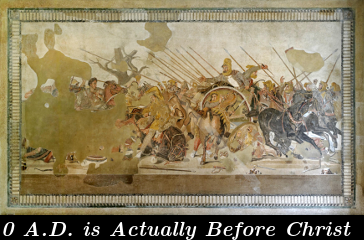
\includegraphics[width=\textwidth]{Alexander}
\end{center}

\clearpage
\tableofcontents

\clearpage
\section{Introduction}
\textbf{0abc} is an acronym for ``0 A.D. is Actually Before Christ''. Of the twelve civilizations and factions included in the default distribution, three (Britons, Gauls, Iberians) cover the whole period (c. 500--1 B.C.), three (Athenians, Persians, Spartans) the Classical period (c. 500--300 B.C.), and six (Carthaginians, Macedonians, Mauryas, Ptolemies, Romans, Seleucids) the Hellenistic period (c. 350--150 B.C.); civilizations (Armenia, Han China, Numidia, Parthia, Pontus, Xiongnu) peaking in the last two centuries (c. 200--1 B.C.) are noticeably lacking. % Iron Age: Assyrians (Neo-Assyrian Empire), Chaldeans (Neo-Babylonian Empire), Etruscans, Kush (Nubia), Lydia, Phrygia, Urartu (Armenia)

This mod, however, does not include any new factions. It tweaks, rebalances, and improves upon what already exists in the game. Amongst other things, it contains a moderate bonus attack counter and penalty system, more experience promotion ranks (0--12), and a new resource (silver).

\textbf{0abc} serves as a showcase for what 0 A.D. easily could be at the moment, as a playground for me experimenting with modifying the game to get used to the code structure, and as a platform for including my own opinions and views to have the game the way I like it. Being a test mod of an alpha-stage game, it is inherently imperfect, unfinished, and restricted by my limited programming skills and the files available in 0 A.D.'s latest stable release. 

All the content is completely open for any use: feel free to download, change, redistribute, or (re)use anything in any way you like; no asking for permission or granting credits is required for incorporating parts or all of it in your own mods (or main distribution). Have fun with it!

%\begin{comment}
\subsection{Instructions}
\begin{itemize}
  \item Use \texttt{git clone} \url{https://github.com/0abc/0abc-a22.git} to get the repository directly or download it as a zip via \url{https://github.com/0abc/0abc-a22/archive/master.zip}
  \item Place it in your \texttt{/0ad/mods/} folder:
  \subitem GNU/Linux (e.g. Fedora) typically: \verb+~/.local/share/0ad/mods/+
  \subitem Macintosh/Apple OS X typically: \verb+~/Library/Application\Support/0ad/mods/+
  \subitem Microsoft Windows typically: \verb+~\Documents\My Games\0ad\mods\+
  \item Launch 0 A.D., click ``Tools \& Options'' and ``Mod Selection''
  \item Select \texttt{0abc}, click ``Enable'' and ``Save Configuration''
  \item Add, remove, or move up or down any other mods, click ``Save Configuration'' and ``Start Mods''
  \item Click ``Learn To Play'' and ``Structure Tree'' to see the mod(s) implemented.
\end{itemize}

\subsection{Intended but not yet implemented}
\begin{itemize}
  \item Units can occupy more than one garrison slot (e.g. infantry one, cavalry two, elephants six).
  \item Domestic animals start at e.g. 20\% of maximum food and gradually fatten to 100\%.
  \item Fruit trees contain both food and wood; right-click to gather food, control-right-click to cut the tree and collect wood; when food is reduced to 0 it does not disappear but stays, allowing it to regrow fruit and be harvested again later; when cutting starts, the tree is killed, does not have any food any more, and completely disappears when all wood is gathered.
  \item Farmstead serves as a dropsite for food.fruit and food.grain (but not food.meat) and corral as a dropsite for food.meat (but not other food types).
  \item Trader gain is 100\% silver; bartering resources is always possible, also without a market.
\end{itemize}

\begin{comment}
\subsection{More factions (not implemented)}
%  \item Replace the basic/advanced/elite rank system with smoother experience upgrades, where all human soldiers (citizen, mercenary, and champion) start at rank 0 and can advance up to rank 12; each rank grants $+5\%$ health, attack damage, and capture rates ($1.05^{12}=1.80$, i.e. a 80\% improvement), but also $-10\%$ resource gather rates ($0.9^{12}=0.28$, i.e. a 72\% reduction); no armour, range, speed, or vision increases; healers acquire $+5\%$ health and HP heal rate per rank. Every phase there is at least one technology available at the barracks which increases the basic rank by one. 
  Add more factions to cover the 8th, 7th, 6h and the 2nd and 1st centuries B.C. (existing factions are indicated with an asterisk (*)):

Armenians (Greater Armenia, 331~BC--428~AD, peaked first half 1st C. BC)
Assyrians (Neo-Assyrian Empire, 911--612), 
Attalids (Pergamon, 282--133),
Britons*,
Carthaginians* (814--146),
Chaldeans (Neo-Babylonian Empire, 626--539),
Epirus (330--167), 
Etruscans (768--264),
Gauls*,
Greeks (c.800--146; subdivided into four factions: Athenians/Athens*, Boeotians/Thebes, Lacedaemonians/Sparta*, and Sicilians/Syracusae)\footnote{Other important local powers included Argos, Milete, and Samos peaking in the Archaic period, Corinth, and Tarentum in the Classical period, and the Acarnanians and Aetolians, Achaeans, and Rhodians peaking in the Hellenistic period.},
Iberians*,
Illyrians,
Lydians (unclear--546),
Macedonians* (Macedon, 808--168, peaked 323), 
Mauryas* (India, 326--180),
Nubians (Kush (Napata, Meroe), 1070~BC--350~AD, peaked c.700 BC),
Numidia (202--40),
Parthians (Arsacid Empire, 247~BC--224~AD, peaked middle 2nd C. BC),
Persians* (Achaemenid Empire, c.550--330),
Phrygians (c.800--c.600),
Pontus (281~BC--66~BC/62~AD, peaked first half 1st C. BC),
Ptolemies* (Egypt, 305--30),
Romans* (Roman Republic, 509--27),
Scythians,
Seleucids* (Syria, 312--63),
Thracians,
Urartu (Armenia, 860--590).
\end{comment}

\subsection{Further information}
People interested in Antiquity are lucky to live nowadays. Thanks to widespread digitization, availability of sources is no longer a problem; the choice of sources is. 
Wikipedia is a mixed blessing which has to be used with care: some articles are much better than corresponding lemmas of paper encyclopaedias, others contain outright rubbish and dangerous nonsense.
\textit{The Cambridge History of Greek and Roman Warfare} (2007) is a decent starting point.
Those without access to a university library and looking for something specific can contact me.\footnote{\url{https://wildfiregames.com/forum/index.php?/profile/21417-nescio/}}



\clearpage
\section{Units}
\subsection{General overview}
\begin{itemize}
  \item All soldiers (except for war dogs) require at least some metal, to encourage feminization.
  \item All soldiers (citizen, mercenary, and champion) can promote up to twelve times; each rank grants $+5\%$ health, attack damage, and capture attack, melee units also receive $+1\%$ movement speed and ranged units $-1\%$ spread.
  \subitem Healers receive $+5\%$ health, $-5\%$ healing time, and $+1$~m healing range every promotion.
  \item Loot is standardized to $0$, experience is equal to the sum of the total costs.
\end{itemize}


\subsubsection{Worker rates}
\begin{tabular}{l|cccccccc}
 & fishing boat & woman & slave & melee infantry & ranged infantry & mercenary & champion & hero \\
\hline
build (structure)   &  --  &  --  & 1.00 & 1.00 & 1.00 & 1.00 &  --  &  --  \\
farm (food.grain)   &  --  & 0.40 & 0.35 & 0.30 & 0.25 &  --  &  --  &  --  \\
fish (food.fish)    & 1.50 & 0.60 & 0.50 & 0.70 & 0.75 &  --  &  --  &  --  \\
forage (food.fruit) &  --  & 1.00 & 0.50 & 0.50 & 0.50 &  --  &  --  &  --  \\
hunt (food.meat)    & 2.00 & 0.80 & 0.80 & 0.90 & 1.00 &  --  &  --  &  --  \\
lumber (wood.tree)  &  --  & 0.50 & 1.00 & 0.70 & 0.70 &  --  &  --  &  --  \\
mine (metal.ore)    &  --  & 0.20 & 0.50 & 0.30 & 0.30 &  --  &  --  &  --  \\
quarry (stone.rock) &  --  & 0.20 & 0.50 & 0.30 & 0.30 &  --  &  --  &  --  \\
\end{tabular}

\subsubsection{Soldier types}
\begin{tabular}{l|ccccccc}
                           & infantry & camel    & cavalry  & biga     & quadriga & elephant \\
                           &          &          &          & chariot  & chariot  &          \\
\hline
population cost            &     1    &     2    &     2    &     4    &     6    &     6    \\
training time              &    20    &    25    &    30    &    35    &    40    &    45    \\
food cost                  &    25    &    60    &    75    &   150    &   250    &   300    \\
food upkeep per 1~s        &     0.02 &     0.04 &     0.05 &     0.10 &     0.15 &     0.20 \\ 
experience to promote      &   100    &   125    &   150    &   200    &   240    &   300    \\
vision range               &    75    &    85    &    80    &    80    &    80    &    90    \\
\hline
mercenary f/w/m/s costs    &   $=0.0$ &   $=0.0$ &   $=0.0$ &   $=0.0$ &   $=0.0$ &   $=0.0$ \\
mercenary silver cost      &   $60.0$ &   $75.0$ &   $90.0$ &  $180.0$ &  $240.0$ &  $300.0$ \\ 
mercenary training time    &  $-50\%$ &  $-50\%$ &  $-50\%$ &  $-50\%$ &  $-50\%$ &  $-50\%$ \\
mercenary health           &  $+10\%$ &  $+10\%$ &  $+10\%$ &  $+10\%$ &  $+10\%$ &  $+10\%$ \\
mercenary armour (h, c, p) &   $+1.0$ &   $+1.0$ &   $+1.0$ &   $+1.0$ &   $+1.0$ &   $+1.0$ \\
mercenary attack damage    &  $+20\%$ &  $+20\%$ &  $+20\%$ &  $+20\%$ &  $+20\%$ &  $+20\%$ \\
mercenary capture strength &   $+0\%$ &   $+0\%$ &   $+0\%$ &   $+0\%$ &   $+0\%$ &   $+0\%$ \\
\hline
veteran metal cost         &  $+30.0$ &  $+40.0$ &  $+50.0$ &  $+70.0$ &  $+80.0$ & $+100.0$ \\
veteran wood cost          &  $+15.0$ &  $+20.0$ &  $+25.0$ &  $+35.0$ &  $+40.0$ &  $+50.0$ \\
veteran training time      &  $+50\%$ &  $+50\%$ &  $+50\%$ &  $+50\%$ &  $+50\%$ &  $+50\%$ \\
veteran health             &  $+20\%$ &  $+20\%$ &  $+20\%$ &  $+20\%$ &  $+20\%$ &  $+20\%$ \\
veteran armour (h, c, p)   &   $+2.0$ &   $+2.0$ &   $+2.0$ &   $+2.0$ &   $+2.0$ &   $+2.0$ \\
veteran attack damage      &  $+50\%$ &  $+50\%$ &  $+50\%$ &  $+50\%$ &  $+50\%$ &  $+50\%$ \\
veteran capture strength   &  $+50\%$ &  $+50\%$ &  $+50\%$ &  $+50\%$ &  $+50\%$ &  $+50\%$ \\
\hline
champion metal cost        &  $+50.0$ &  $+60.0$ &  $+70.0$ & $+100.0$ & $+120.0$ & $+150.0$ \\
champion wood cost         &  $+25.0$ &  $+30.0$ &  $+35.0$ &  $+50.0$ &  $+60.0$ &  $+75.0$ \\
champion training time     & $+100\%$ & $+100\%$ & $+100\%$ & $+100\%$ & $+100\%$ & $+100\%$ \\
champion health            &  $+50\%$ &  $+50\%$ &  $+50\%$ &  $+50\%$ &  $+50\%$ &  $+50\%$ \\
champion armour (h, c, p)  &   $+3.0$ &   $+3.0$ &   $+3.0$ &   $+3.0$ &   $+3.0$ &   $+3.0$ \\
champion attack damage     & $+100\%$ & $+100\%$ & $+100\%$ & $+100\%$ & $+100\%$ & $+100\%$ \\
champion capture strength  & $+100\%$ & $+100\%$ & $+100\%$ & $+100\%$ & $+100\%$ & $+100\%$ \\
%\hline
%hero metal cost            & $+400\%$ & $+400\%$ & $+400\%$ & $+400\%$ & $+400\%$ & $+400\%$ & $+400\%$ \\
%hero wood cost             & $+400\%$ & $+400\%$ & $+400\%$ & $+400\%$ & $+400\%$ & $+400\%$ & $+400\%$ \\
%hero resource cost         & $+400\%$ & $+400\%$ & $+400\%$ & $+400\%$ & $+400\%$ & $+400\%$ & $+400\%$ \\
%hero health                & $+900\%$ & $+900\%$ & $+900\%$ & $+900\%$ & $+900\%$ & $+900\%$ & $+900\%$ \\
%hero armour (h, c, p)      &   $+5.0$ &   $+5.0$ &   $+5.0$ &   $+5.0$ &   $+5.0$ &   $+5.0$ &   $+5.0$ \\
%hero attack damage         & $+400\%$ & $+400\%$ & $+400\%$ & $+400\%$ & $+400\%$ & $+400\%$ & $+400\%$ \\
%hero capture strength      & $+400\%$ & $+400\%$ & $+400\%$ & $+400\%$ & $+400\%$ & $+400\%$ & $+400\%$ \\
\end{tabular}


\textbf{NB:} Champions also require twice as much experience to advance in rank. Other unit statistic bonuses are removed. % Citizen soldiers are 100\%. 

\begin{comment}
\subsubsection{Unit categories}
\begin{tabular}{l|cccccc}
 & {\bf population} & {\bf standard} & {\bf resource} & {\bf worker} & {\bf vision} & {\bf promotion  } \\
 & {\bf slots     } & {\bf food    } & {\bf carry   } & {\bf gather} & {\bf range } & {\bf experience } \\
 & {\bf occupied  } & {\bf cost    } & {\bf capacity} & {\bf rate  } & {(metres)  } & {\bf requirement} \\
\hline
War dogs                        & 0 &  30 & -- &  -- & 60 &  75 \\
Healers                         & 1 &  25 & -- &  -- & 60 & 250 \\
Infantry                        & 1 &  25 & 10 & 1.0 & 75 & 100 \\
Camels                          & 2 &  40 & 40 & 1.8 & 85 & 125 \\
Cavalry                         & 2 &  50 & 30 & 2.0 & 80 & 150 \\
Bigae (two-horse chariots)      & 4 & 100 & 60 & 3.6 & 80 & 200 \\
Quadrigae (four-horse chariots) & 6 & 150 & 60 & 3.6 & 80 & 240 \\
War elephants                   & 6 & 200 & 75 & 3.0 & 90 & 300 \\
\end{tabular}
\subsection{Infantry}
\begin{itemize}
  \item All unit categories inflict bonus damage against at least one unit class;
  \subitem Crush damage soldiers (macemen, slingers) have a 75\% penalty vs structures; Mauryas can construct rams;
  \subitem Archers have a 50\% penalty vs elephants.
\end{itemize}

\subsection{Mounted}
\begin{itemize}
  \item Camelry, chariotry, and elephantry are now separate unit categories, independent of cavalry.
  \subitem As a consequence, they no longer benefit from Cavalry technologies (e.g. blacksmith's cavalry armour researches).
  \item All unit categories (except melee elephants) inflict bonus damage against at least one unit class;
  \subitem Archers, camels, and chariots have a 50\% penalty vs elephants;
  \subitem Melee cavalry has a 50\% penalty vs elephants and a 25\% penalty vs camels and chariots;
  \subitem Crush damage soldiers (melee elephants) have a 75\% penalty vs structures.
  \item Elephants can garrison up to 3 infantry units
\end{itemize}

\subsubsection{Factions}
\begin{itemize}
  \item Athenians can construct gymnasium in town phase.
  \item Ptolemies can construct a theatre; lighthouse requires city phase; start with slingers in village phase; infantry skirmishers are now town phase mercenaries.
  \item Romans can train new \textit{principes} (experienced swordsmen) in addition to slightly weakened \textit{hastati} (young swordsmen); both are available in village phase (at the barracks and the army camp).
  \item Seleucids can construct a theatre.
  \item Spartans can construct (stone) city walls; can no longer construct theatre.
  \item Mauryan elephant archers can shoot one additional arrow per archer garrisoned (up to five)
  \item Persians have Dahae horse archers (using Seleucid graphics) as their Town phase cavalry archers (instead of Babylonian chariots)
  \item Persians can train Babylonian scythed chariot champions at the Stables in the City phase
\end{itemize}
\end{comment}


\begin{landscape}
\subsection{Unit statistics comparison tables}
\textbf{NB:} The new values are displayed normally, the default ``0 A.D. Alpha XXII: Venustas'' values are displayed for comparison between brackets ().

\subsubsection{Infantry units}
\begin{tabular}{l|ccc|cccc|ccc|l}
{\bf class} & {\bf pop.} & {\bf training costs} & {\bf loot}          & {\bf vision} & {\bf speed} & {\bf health} & {\bf armour} & {\bf damage} & {\bf range} & {\bf rate} & {\bf counters/} \\
            & {\bf size} & {(f, w, m, s; time)} & {(f, w, m, s; exp)} & {\bf range}  &             &              & {(h, p, c)}  & {(h, p, c)}  & {(m)}       & {(ms)}     & {\bf penalties} \\
\hline
war dog                            &  0  &  30,  0,  0, 0; 15  &  0, 0, 0, 0;  30  &  60  &    15+15    &   75  &   1,  1,  1  &  0,  5,  0  &   3  &  1000  & $0.75\times$ vs Camelry, Cavalry,\\
(non-human)                        & (0) & (100, 0,  0, 0; 15) & (10, 0,0, 0; 100) & (30) & (14.5+11.5) &  (90) &  (1,  2,  1) & (7,  2,  0) &  (3) & (1000) & Chariotry, $0.5\times$ vs Elephantry\\
\hline
infantry                           &  1  &  25, 30, 20, 0; 20  &  0, 0, 0, 0;  60  &  75  &     9+11    &   50  &   2,  3,  1  &  0,  4,  2  &  60  &  1000  & $1.5\times$ vs Cavalry Archers \\
crossbowman\textsuperscript{2}     & (1) & (50, 50,  0, 0; 10) & (5, 5, 0, 0; 100) & (80) &    (8+10)   &  (50) &  (1,  1, 10) & (0,  6,  0) & (72) & (1000) & $0.5\times$ vs Elephantry \\
\hline
infantry                           &  1  &  25, 35, 15, 0; 20  &  0, 0, 0, 0;  60  &  75  &    11+9     &   50  &   3,  2,  1  &  0,  6,  0  &  60  &  1000  & $1.5\times$ vs Cavalry Archers \\
archer                             & (1) & (50, 50,  0, 0; 10) & (5, 5, 0, 0; 100) & (80) &    (8+10)   &  (50) &  (1,  1, 10) & (0,  6,  0) & (72) & (1000) & $0.5\times$ vs Elephantry \\
\hline
infantry                           &  1  &  25, 45,  5, 0; 20  &  0, 0, 0, 0;  60  &  75  &    11+9     &   50  &   2,  1,  3  &  0,  5,  0  &  60  &  1000  & $1.5\times$ vs Cavalry Archers \\
longbowman\textsuperscript{1}      & (1) & (50, 50,  0, 0; 10) & (5, 5, 0, 0; 100) & (80) &    (8+10)   &  (50) &  (1,  1, 10) & (0,  6,  0) & (72) & (1000) & $0.5\times$ vs Elephantry \\
\hline
infantry                           &  1  &  25, 30, 0, 20; 20  &  0, 0, 0, 0;  60  &  75  &    12+8     &   55  &   1,  3,  2  &  0,  4,  4  &  45  &  1000  & $1.5\times$ vs Infantry Archers\\
slinger                            & (1) & (50, 20, 0, 30; 10) & (5, 0, 0, 5; 100) & (80) &   (11+13)   &  (50) &  (1,  1, 10) & (0, 9.5, 1) & (48) & (1000) & $0.125\times$ vs Structures, Siege\\
\hline
infantry                           &  1  &  25, 40, 10, 0; 20  &  0, 0, 0, 0;  60  &  75  &    13+7     &   60  &   1,  2,  3  &  0, 10,  0  &  30  &  1000  & \\
javelinist                         & (1) & (50, 50,  0, 0; 10) & (5, 5, 0, 0; 100) & (80) & (13.5+10.5) &  (50) &  (1,  1, 10) & (0, 16,  0) & (24) & (1250) & \\
\hline
infantry                           &  1  &  25, 30, 20, 0; 20  &  0, 0, 0, 0;  60  &  75  &    10+10    &   65  &   2,  2,  2  &  8,  0,  2  &  15  &  1000  & \\
axe thrower\textsuperscript{2}     & (1) & (50, 50,  0, 0; 10) & (5, 5, 0, 0; 100) & (80) & (13.5+10.5) &  (50) &  (1,  1, 10) & (0, 16,  0) & (24) & (1250) & \\
\hline
infantry                           &  1  &  25, 40, 10, 0; 20  &  0, 0, 0, 0;  60  &  75  &    11+9     &   85  &   4,  6,  5  & 4.8, 0, 1.2 &   2  &  1000  & $1.5\times$ vs Elephantry\\
axeman\textsuperscript{1}          & (1) & (50, 40, 10, 0; 10) & (5, 5, 0, 0; 100) & (80) &  (9.5+6.5)  & (100) &  (5,  5, 15) & (5.5, 0, 0) &  (2) &  (750) & \\
\hline
infantry                           &  1  &  25, 35, 15, 0; 20  &  0, 0, 0, 0;  60  &  75  &    10+10    &   90  &   5,  5,  5  &  0,  0,  6  &   2  &  1000  & $0.125\times$ vs Structures\\
maceman\textsuperscript{1}         & (1) & (50, 40, 10, 0; 10) & (5, 0, 5, 0; 100) & (80) &  (9.5+6.5)  & (100) &  (5,  5, 15) & (0, 0, 5.5) &  (2) &  (750) & \\
\hline
infantry                           &  1  &  25, 30, 20, 0; 20  &  0, 0, 0, 0;  60  &  75  &    10+10    &   95  &   5,  4,  6  & 4.8, 1.2, 0 &   2  &  1000  & -- \\
sabreman\textsuperscript{1}        & (1) & (50, 40, 10, 0; 10) & (5, 0, 5, 0; 100) & (80) &  (9.5+6.5)  & (100) &  (5,  5, 15) & (5.5, 0, 0) &  (2) &  (750) & \\
\hline
infantry                           &  1  &  25, 25, 25, 0; 20  &  0, 0, 0, 0;  60  &  75  &     9+11    &   95  &   6,  5,  4  &  4,  2,  0  &   2  &  1000  & -- \\
swordsman                          & (1) & (50, 40, 10, 0; 10) & (5, 0, 5, 0; 100) & (80) &  (9.5+6.5)  & (100) &  (5,  5, 15) & (5.5, 0, 0) &  (2) &  (750) & \\
\hline
infantry                           &  1  &  25, 20, 30, 0; 20  &  0, 0, 0, 0;  60  &  75  &    10+10    &   95  &   6,  4,  5  & 4.5, 1.5, 0 &   3  &  1000  & -- \\
longswordsman\textsuperscript{1}   & (1) & (50, 40, 10, 0; 10) & (5, 0, 5, 0; 100) & (80) &  (9.5+6.5)  & (100) &  (5,  5, 15) & (5.5, 0, 0) &  (2) &  (750) & \\
\hline
infantry                           &  1  &  25, 35, 15, 0; 20  &  0, 0, 0, 0;  60  &  75  &    10+10    &   85  &   5,  5,  5  &  3,  3,  0  &   3  &  1000  & -- \\
halberdier\textsuperscript{2}      & (1) & (50, 50,  0, 0; 10) & (5, 5, 0, 0; 100) & (80) &    (7+2)    & (100) & (10, 10, 15) & (1,  3,  0) &  (8) & (2000) & \\
\hline
infantry                           &  1  &  25, 40, 10, 0; 20  &  0, 0, 0, 0;  60  &  75  &     9+11    &   90  &   4,  5,  6  &  1,  5,  0  &   4  &  1000  & -- \\
spearman                           & (1) & (50, 50,  0, 0; 10) & (5, 5, 0, 0; 100) & (80) &  (8.5+6.5)  & (100) &  (5,  5, 15) & (3, 2.5, 0) &  (4) & (1000) & \\
\hline
infantry                           &  1  &  25, 25, 25, 0; 20  &  0, 0, 0, 0;  60  &  75  &     7+13    &  100  &   5,  6,  4  & 1.2, 4.8, 0 &   4  &  1000  & -- \\
hoplite\textsuperscript{1}         & (1) & (50, 50,  0, 0; 10) & (5, 5, 0, 0; 100) & (80) &  (8.5+6.5)  & (100) &  (5,  5, 15) & (3, 2.5, 0) &  (4) & (1000) & \\
\hline
infantry                           &  1  &  25, 45,  5, 0; 20  &  0, 0, 0, 0;  60  &  75  &     8+12    &   80  &   3,  5,  7  &  0,  6,  0  &   6  &  1000  & -- \\
pikeman                            & (1) & (50, 50,  0, 0; 10) & (5, 5, 0, 0; 100) & (80) &    (7+2)    & (100) & (10, 10, 15) & (1,  3,  0) &  (8) & (2000) & \\
\end{tabular}

\textbf{NB}:
%\textbf{0}: Replaces the default $3.0\times$ vs Cavalry bonus\\
\textbf{1}: A new class to which existing units are reassigned;
\textbf{2}: A new class which currently remains unused


\clearpage
\subsubsection{Mounted units}
\begin{tabular}{l|ccc|cccc|ccc|l}
{\bf class} & {\bf pop.} & {\bf training costs} & {\bf loot}          & {\bf vision} & {\bf speed} & {\bf health} & {\bf armour} & {\bf damage} & {\bf range} & {\bf rate} & {\bf counters/} \\
            & {\bf size} & {(f, w, m, s; time)} & {(f, w, m, s; exp)} & {\bf range } &             &              & {(h, p, c)}  & {(h, p, c)}  & {(m)}       & {(ms)}     & {\bf penalties} \\
\hline
camel                                 &  2  &   60,  35,  15, 0; 25  &  0,  0,  0,  0;  90  &   85  &    25+10    &  108  &   1,  1,  1  &   0, 6.5, 0  &  68  &  1000  & $1.5\times$ vs Traders\\
archer\textsuperscript{1}             & (1) & (100,  40,   0, 0; 12) & (10,  0,  5, 0; 130) &  (92) & (17.5+10.5) & (120) &  (3,  1, 15) &  (0,  7,  0) & (72) & (1000) & $0.5\times$ vs Elephantry\\
\hline
camel                                 &  2  &   60,  40,  10, 0; 25  &  0,  0,  0,  0;  90  &   85  &    26+9     &  117  &   1,  1,  1  &   0, 11,  0  &  34  &  1000  & $1.5\times$ vs Chariotry\\
javelinist\textsuperscript{2}         & (1) & (100,  40,   0, 0; 12) & (10,  0,  5, 0; 130) &  (92) & (17.5+10.5) & (120) &  (3,  1, 15) &  (0, 18,  0) & (28) & (1250) & -- \\
\hline
camel                                 &  2  &   60,  40,  10, 0; 25  &  0,  0,  0,  0;  90  &   85  &    27+8     &  144  &   2,  2,  2  &   0,  7,  0  &   5  &  1000  & $1.5\times$ vs Cavalry\\
spearman\textsuperscript{2}           & (1) &  (80,  55,   0, 0; 12) & (10,  0,  5, 0; 130) &  (92) &   (22+18)   & (160) &  (1,  1, 10) &  (6, 13,  0) &  (6) & (3500) & $0.5\times$ vs Elephantry\\
\hline
cavalry                               &  2  &   75,  30,  20, 0; 30  &  0,  0,  0,  0; 120  &   80  &    16+14    &  110  &   1,  1,  1  &   0,  5, 2.5 &  64  &  1000  & $1.25\times$ vs Cavalry \\
crossbowman\textsuperscript{2}        & (1) & (100,  40,   0, 0; 12) & (10,  0,  5, 0; 130) &  (92) & (17.5+10.5) & (120) &  (3,  1, 15) &  (0,  7,  0) & (72) & (1000) & $0.5\times$ vs Elephantry\\ % $0.125\times$ vs Structures
\hline
cavalry                               &  2  &   75,  35,  15, 0; 30  &  0,  0,  0,  0; 120  &   80  &    22+8     &  120  &   1,  1,  1  &   0,  7,  0  &  64  &  1000  & $1.5\times$ vs Cavalry Axe-, Sabre-, and Swordsmen\\
archer                                & (1) & (100,  40,   0, 0; 12) & (10,  0,  5, 0; 130) &  (92) & (17.5+10.5) & (120) &  (3,  1, 15) &  (0,  7,  0) & (72) & (1000) & $0.5\times$ vs Elephantry\\
\hline
cavalry                               &  2  &   75,  40,  10, 0; 30  &  0,  0,  0,  0; 120  &   80  &    21+9     &  130  &   1,  1,  1  &   0, 12,  0  &  32  &  1000  & $1.5\times$ vs Chariotry\\
javelinist                            & (1) & (100,  40,   0, 0; 12) & (10,  0,  5, 0; 130) &  (92) & (17.5+10.5) & (120) &  (3,  1, 15) &  (0, 18,  0) & (28) & (1250) & -- \\
\hline
cavalry                               &  2  &   75,  35,  15, 0; 30  &  0,  0,  0,  0; 120  &   80  &    20+10    &  140  &   3,  3,  3  &  6,  0, 1.5  &   4  &  1000  & $0.75\times$ vs Camelry, Chariotry;\\
axeman\textsuperscript{1}             & (1) &  (80,  35,  20, 0; 12) & (10,  0,  5, 0; 130) &  (92) &   (20+8.75) & (160) &  (4,  2, 15) & (6.5, 0,  0) &  (6) &  (750) & $0.5\times$ vs Elephantry\\
\hline
cavalry                               &  2  &   75,  25,  25, 0; 30  &  0,  0,  0,  0; 120  &   80  &    19+11    &  150  &   3,  3,  3  &  6, 1.5,  0  &   4  &  1000  & $0.75\times$ vs Camelry, Chariotry;\\
sabreman                              & (1) &  (80,  35,  20, 0; 12) & (10,  0,  5, 0; 130) &  (92) &   (20+8.75) & (160) &  (4,  2, 15) & (6.5, 0,  0) &  (6) &  (750) & $0.5\times$ vs Elephantry\\
\hline
cavalry                               &  2  &   75,  25,  25, 0; 30  &  0,  0,  0,  0; 120  &   80  &    19+11    &  150  &   3,  3,  3  &  5, 2.5,  0  &   4  &  1000  & $0.75\times$ vs Camelry, Chariotry;\\
swordsman                             & (1) &  (80,  35,  20, 0; 12) & (10,  0,  5, 0; 130) &  (92) &   (20+8.75) & (160) &  (4,  2, 15) & (6.5, 0,  0) &  (6) &  (750) & $0.5\times$ vs Elephantry\\
\hline
cavalry                               &  2  &   75,  30,  20, 0; 30  &  0,  0,  0,  0; 120  &   80  &    18+12    &  160  &   3,  3,  3  &  1.5, 6,  0  &   4  &  1000  & $0.75\times$ vs Camelry, Chariotry;\\
spearman                              & (1) &  (80,  55,   0, 0; 12) & (10,  0,  5, 0; 130) &  (92) &   (22+18)   & (160) &  (4,  3, 15) &  (6, 13,  0) &  (6) & (3500) & $0.5\times$ vs Elephantry\\
\hline
cavalry                               &  2  &   75,  20,  30, 0; 30  &  0,  0,  0,  0; 120  &   80  &    17+13    &  170  &   3,  3,  3  &  0,   7,  1  &   4  &  1000  & $0.75\times$ vs Camelry, Chariotry;\\
lancer\textsuperscript{1}             & (1) &  (80,  55,   0, 0; 12) & (10,  0,  5, 0; 130) &  (92) &   (22+18)   & (160) &  (4,  3, 15) &  (6, 13,  0) &  (6) & (3500) & $0.5\times$ vs Elephantry\\
\hline
archer                                &  4  &  150,  90,  35, 0; 35  &  0,  0,  0,  0; 240  &   80  &    16+9     &  250  &   6,  6,  6  &   0, 10,  0  &  64  &  1000  & -- \\% $1.5\times$ vs Mace Infantry\\
biga chariot\textsuperscript{1,3}     & (1) & (250, 100, 100, 0; 40) & (10, 10, 20, 0; 150) &  (96) & (20.5+7.5)  & (270) &  (7,  5, 20) &  (0, 14,  0) & (76) & (1000) & $0.5\times$ vs Elephantry\\
\hline
javelin                               &  4  &  150, 100,  25, 0; 35  &  0,  0,  0,  0; 240  &   80  &    16+9     &  270  &   6,  6,  6  &   0, 20,  0  &  32  &  1000  & -- \\%$1.5\times$ vs Sword Infantry\\ 
biga chariot\textsuperscript{1,3}     & (1) & (250, 100, 100, 0; 40) & (10, 10, 20, 0; 150) &  (96) & (20.5+7.5)  & (270) &  (7,  5, 20) &  (0, 36,  0) & (32) & (1250) & $0.5\times$ vs Elephantry\\
\hline
scythed                               &  6  &  250, 100,  50, 0; 40  &  0,  0,  0,  0; 300  &   80  &    18+9     &  360  &   6,  6,  6  &   0, 12,  0  &  64  &  1000  & -- \\% $1.5\times$ vs Spear Infantry\\
quadriga chariot\textsuperscript{1,3} & (1) & (250, 100, 100, 0; 40) & (10, 10, 20, 0; 150) &  (96) & (20.5+7.5)  & (270) &  (7,  5, 20) &  (0, 14,  0) & (76) & (1000) & $0.5\times$ vs Elephantry\\
\hline
archer                                &  6  &  300, 100, 100, 0; 45  &  0,  0,  0,  0; 360  &   90  &    10+10    &  450  &   2,  6,  4  &   0,  8,  0  &  72  &  1000  & -- \\
elephant\textsuperscript{1}           & (1) & (200,  80,  20, 0; 12) & (25, 10,  5, 0; 260) &  (92) &  (8.5+5.5)  & (240) &  (4,  3, 15) & (0, 10.5, 0) & (72) &  (750) & $0.5\times$ vs Elephantry\\
\hline
melee war                             &  6  &  300,  50, 100, 0; 45  &  0,  0,  0,  0; 360  &   90  &    10+10    &  500  &   4,  8,  6  &   0,  0, 30  &   6  &  1000  & -- \\
elephant\textsuperscript{1,3}         & (3) & (250,   0, 250, 0; 30) & (10, 10, 20, 0; 150) & (100) &  (8.5+5.5)  & (750) & (10, 10, 25) & (20, 0, 150) &  (8) & (1500) & $0.125\times$ vs Structures\\
\end{tabular}

\textbf{NB}:
\textbf{1}: A new class to which existing units are reassigned;\\
\textbf{2}: A new class which currently remains unused;\\
\textbf{3}: Comparison values are champions % A new class to which exclusively champion units are reassigned; default values not %; keep in mind all champions have $+50\%$ health, $+3$ armour levels, and $+100\%$ attack, as well as $+50$ wood and $+100$ metal in costs, $+150\%$ training time, and $+5$ wood, $+10$ metal, and $+150$ experience in loot


\clearpage
\subsubsection{Ships}
\begin{tabular}{l|ccc|ccccc|cccc}
{\bf class} & {\bf pop.} & {\bf training costs} & {\bf loot}          & {\bf garrison} & {\bf vision} & {\bf speed} & {\bf health/} & {\bf armour} & {\bf damage} & {\bf range} & {\bf rate} & {\bf arrow} \\
            & {\bf size} & {(f, w, m, s; time)} & {(f, w, m, s; exp)} & {\bf capacity} & {\bf range}  &             & {\bf capture} & {(h, p, c)}  & {(h, p, c)}  & {(m)}       & {(ms)}     & {\bf count} \\
\hline % all:
fishing boat          &  0  &   10,  40,   0,   0; 10  &  0,  0,  0,  0;    0  &    1  &   60  &    10+2    &   150/--  &   2,  4,  2  &   10,   0,   0  &   5  &  1000  &   --    \\ (resource gatherer)
                      & (1) &   (0,  50,   0,   0; 20) & (0, 10,  0,  0;    1) &   (1) &  (24) &   (10+0)   &  (200/--) &  (2,  5,  2) &  (10,   0,   0) &  (5) & (1000) &  (--)   \\
\hline % all:
merchant ship         &  0  &   25, 150,  50,   0; 20  &  0,  0,  0,  0;    0  &   15  &   75  &    12+3    &   600/--  &   3,  6,  3  &        --       &  --  &   --   &   --    \\ (trader)
                      & (1) &   (0,   0, 100,   0; 20) & (0, 15,  0,  0;   25) &  (15) &  (50) &   (12+0)   &  (400/--) &  (2,  5,  2) &       (--)      & (--) &  (--)  &  (--)   \\
\hline % unused:
small barge           &  0  &   50, 100,  50,   0; 15  &  0,  0,  0,  0;   90  &   10  &  100  &    14+4    &   450/--  &   4,  8,  4  &    0,  12,   0  &  60  &  1000  &  2--5   \\ (transport)
\textsuperscript{2}   & (3) &   (0, 150, 150,   0; 40) & (0, 30, 20,  0;  100) &  (40) &  (90) &   (14+4)   & (1600/--) &  (5, 10,  5) &   (0,  25,   0) & (55) & (2000) & (3--13) \\ 
\hline % maur:
medium barge          &  0  &   50, 200,  50,   0; 20  &  0,  0,  0,  0;  180  &   20  &  100  &    14+4    &   900/--  &   5, 10,  5  &    0,  12,   0  &  60  &  1000  &  2--8   \\ (transport)
\textsuperscript{1}   & (3) &   (0, 150, 150,   0; 40) & (0, 30, 20,  0;  100) &  (40) &  (90) &   (14+4)   & (1600/--) &  (5, 10,  5) &   (0,  25,   0) & (55) & (2000) & (3--13) \\ 
\hline % brit, gaul, iber, maur:
large barge           &  0  &   50, 400,  50,   0; 25  &  0,  0,  0,  0;  360  &   40  &  100  &    14+4    &  1800/--  &   6, 12,  6  &    0,  12,   0  &  60  &  1000  &  2--14  \\ (transport)
\textsuperscript{1}   & (3) &   (0, 150, 150,   0; 40) & (0, 30, 20,  0;  100) &  (40) &  (90) &   (14+4)   & (1600/--) &  (5, 10,  5) &   (0,  25,   0) & (55) & (2000) & (3--13) \\ 
\hline % unused:
huge barge            &  0  &   50, 800,  50,   0; 30  &  0,  0,  0,  0;  720  &   80  &  100  &    14+4    &  3600/--  &   7, 14,  7  &    0,  12,   0  &  60  &  1000  &  2--26  \\ (transport)
\textsuperscript{2}   & (3) &   (0, 150, 150,   0; 40) & (0, 30, 20,  0;  100) &  (40) &  (90) &   (14+4)   & (1600/--) &  (5, 10,  5) &   (0,  25,   0) & (55) & (2000) & (3--13) \\ 
\hline % iber:
fire ship             &  0  &    0, 150,   0,   0; 15  &           --          &    0  &   60  &    20+0    &   450/--  &   5, 10,  5  &    5,   5,   5  &  10  &   100  &   --    \\ (floating bonfire)
                      & (1) &   (0, 300,   0,   0; 30) &          (--)         &   (0) &  (60) & (17.5+4.5) &  (500/--) &  (5, 10,  5) &  (10,  10,  10) &  (8) &  (100) &  (--)   \\ % -6.0 regeneration
\hline % mace, rome:
skiff                 &  0  &   60,  60,  30,   0; 10  &  0,  0,  0,  0;   60  &    6  &  100  &    18+2    &   300/--  &   5, 10,  5  &    0,  12,   0  &  60  &  1000  &  1--3   \\ (small galley)
\textsuperscript{1}   & (2) &   (0, 125,  50,   0; 20) & (0, 25, 15,  0;   75) &  (20) &  (90) &   (14+4)   &  (800/--) &  (5, 10,  5) &   (0,  35,   0) & (45) & (2000) & (2--10) \\ 
\hline % athen, maur, pers, rome, spart:
unireme               &  0  &  100, 100,  50,   0; 15  &  0,  0,  0,  0;  100  &   10  &  100  &    17+3    &   500/--  &   5, 10,  5  &    0,  12,   0  &  60  &  1000  &  1--4   \\ (light galley)
\textsuperscript{1}   & (2) &   (0, 125,  50,   0; 20) & (0, 25, 15,  0;   75) &  (20) &  (90) &   (14+4)   &  (800/--) &  (5, 10,  5) &   (0,  35,   0) & (45) & (2000) & (2--10) \\
\hline % cart, ptol, sele:
bireme                &  0  &  200, 200, 100,   0; 20  &  0,  0,  0,  0;  200  &   20  &  100  &    16+4    &  1000/--  &   6, 12,  6  &    0,  12,   0  &  60  &  1000  &  2--8   \\ (medium galley)
                      & (2) &   (0, 125,  50,   0; 20) & (0, 25, 15,  0;   75) &  (20) &  (90) &   (14+4)   &  (800/--) &  (5, 10,  5) &   (0,  35,   0) & (45) & (2000) & (2--10) \\
\hline % athen, cart, mace, pers, rome, spart:
trireme               &  0  &  300, 300, 150,   0; 30  &  0,  0,  0,  0;  300  &   30  &  100  &    15+5    &  1500/--  &   6, 12,  6  &    0,  12,   0  &  60  &  1000  &  3--12  \\ (medium galley)
                      & (3) &   (0, 150, 150,   0; 25) & (0, 30, 20,  0;  100) &  (30) &  (90) &   (16+4)   & (1400/--) &  (5, 10,  5) &   (0,  35,   0) & (55) & (2000) & (3--13) \\
\hline % cart, ptol, sele:
quadrireme            &  0  &  400, 400, 200,   0; 40  &  0,  0,  0,  0;  400  &   40  &  100  &    14+6    &  2000/--  &   6, 12,  6  &    0,  12,   0  &  60  &  1000  &  4--16  \\ (medium galley)
\textsuperscript{2}   & (3) &   (0, 150, 150,   0; 25) & (0, 30, 20,  0;  100) &  (30) &  (90) &   (16+4)   & (1400/--) &  (5, 10,  5) &   (0,  35,   0) & (55) & (2000) & (3--13) \\
\hline  % cart, mace, rome, sele:
quinquereme           &  0  &  500, 500, 250,   0; 50  &  0,  0,  0,  0;  500  &   50  &  100  &    13+7    &  2500/--  &   7, 14,  7  &    0,  12,   0  &  60  &  1000  &  5--20  \\ (heavy galley)
                      & (3) &   (0, 350, 200, 350; 30) & (0, 40, 30,  0;  150) &  (50) & (110) &   (16+4)   & (2000/--) &  (5, 10,  5) &   (0,  10, 100) & (10--72) & (5000) & (1--10) \\
\hline % ptol: 
sexireme              &  0  &  600, 600, 300,   0; 60  &  0,  0,  0,  0;  600  &   60  &  100  &    12+8    &  3000/--  &   7, 14,  7  &    0,  12,   0  &  60  &  1000  &  6--24  \\ (heavy galley)
\textsuperscript{1}   & (3) &   (0, 350, 200, 350; 30) & (0, 40, 30,  0;  150) &  (50) & (110) &   (16+4)   & (2000/--) &  (5, 10,  5) &   (0,  10, 100) & (10--72) & (5000) & (1--10) \\
\hline % mace:
septireme             &  0  &  700, 700, 350,   0; 70  &  0,  0,  0,  0;  700  &   70  &  100  &    11+9    &  3500/--  &   7, 14,  7  &    0,  12,   0  &  60  &  1000  &  7--28  \\ (heavy galley)
\textsuperscript{1}   & (3) &   (0, 350, 200, 350; 30) & (0, 40, 30,  0;  150) &  (50) & (110) &   (16+4)   & (2000/--) &  (5, 10,  5) &   (0,  10, 100) & (10--72) & (5000) & (1--10) \\
\hline % ptol:
octoreme              &  0  &  800, 800, 400,   0; 80  &  0,  0,  0,  0;  800  &   80  &  100  &    10+10   &  4000/--  &   8, 16,  8  &    0,  12,   0  &  60  &  1000  &  8--32  \\ (juggernaut galley)
\textsuperscript{1}   & (3) &   (0, 350, 200, 350; 30) & (0, 50, 50,  0;  200) &  (50) & (110) &   (16+4)   & (2000/--) &  (5, 10,  5) &   (0,  10, 100) & (10--72) & (5000) & (1--10) \\
\hline % unused:
novireme              &  0  &  900, 900, 450,   0; 90  &  0,  0,  0,  0;  900  &   90  &  100  &     9+11   &  4500/--  &   8, 16,  8  &    0,  12,   0  &  60  &  1000  &  9--36  \\ (juggernaut galley)
\textsuperscript{2}   & (3) &   (0, 350, 200,   0; 30) & (0, 50, 50,  0;  200) &  (50) & (110) &   (16+4)   & (2000/--) &  (5, 10,  5) &   (0,  10, 100) & (10--72) & (5000) & (1--10) \\
\hline % ptol:
decereme              &  0  & 1000, 1000, 500,  0; 100 &  0,  0,  0,  0; 1000  &  100  &  100  &     8+12   &  5000/--  &   8, 16,  8  &    0,  12,   0  &  60  &  1000  & 10--40  \\ (juggernaut galley)
\textsuperscript{1}   & (8) &   (0, 400, 300, 350; 20) & (0, 50, 50,  0;  200) & (100) &  (90) &   (16+4)   & (4000/--) &  (5, 10,  5) &   (0,  10, 100) & (10--72) & (5000) & (1--10) \\
\end{tabular}

\textbf{NB}: All ships are bribable (espionage); fishing boats and merchant ships are no longer ``conquest critical''.\\
% Juggernauts and heavy warships are city phase, other warships and merchant ships are town phase, and fishing boats are village phase (\emph{all unchanged}).\\
\textbf{1}: A new class to which existing units are reassigned;
\textbf{2}: A new class which currently remains unused


\subsubsection{Siege weapons}
\begin{tabular}{l|ccc|cccc|ccc|l}
{\bf class}    & {\bf pop.} & {\bf training costs} & {\bf loot}          & {\bf vision range} & {\bf speed} & {\bf health} & {\bf armour} & {\bf damage} & {\bf range} & {\bf rate} & {\bf other} \\
{un/pack (ms)} & {\bf size} & {(f, w, m, s; time)} & {(f, w, m, s; exp)} & {packed/unpacked}  &             &              & {(h, p, c)}  & {(h, p, c)}  & {(m)}       & {(ms)}     & {\bf stats} \\
\hline
scorpion      &  1  &  50,  75,  75,   0; 10  &  0,  0,  0,  0; 100  & 50/100&    9+2    &  100  &  1, 10, 1  &  0,  20,   0  &   5--90  &  1000  & -- \\
 6000 (5000)  & (2) &  (0, 250, 250,   0; 20) & (0, 10, 10,  0; 200) & (120) &   (8+4)   & (200) & (1, 50, 5) & (0, 180,  13) &  (8--88) & (4000) & (linear splash damage \\
              &     &                         &                      &       &           &       &            &               &          &        & removed: 0h+75p+5c) \\
\hline
bolt shooter  &  2  & 100, 150, 150,   0; 20  &  0,  0,  0,  0; 200  & 50/100&    8+2    &  200  &  1, 20, 2  &  0,  40,   0  &  10--90  &  1000  & $1.5\times$ vs Elephantry \\
 9000 (10000) & (2) &  (0, 250, 250,   0; 20) & (0, 10, 10,  0; 200) & (120) &   (8+4)   & (200) & (1, 50, 5) & (0, 150,  25) &  (8--80) & (4000) & (linear splash damage \\
              &     &                         &                      &       &           &       &            &               &          &        & removed: 0h+75p+5c) \\
\hline
stone thrower &  3  & 100, 200, 100,   0; 30  &  0,  0,  0,  0; 300  & 50/100&    7+2    &  300  &  1, 30, 3  &  0,   0,  30  &  15--90  &  1000  & $2.0\times$ vs Ships \\
12000 (10000) & (2) &  (0, 400,   0, 250; 25) & (0, 20,  0, 10; 300) & (120) &   (7+3)   & (250) & (1, 50, 5) & (0,  10, 100) & (12--80) & (5000) & circular splash damage: \\
              &     &                         &                      &       &           &       &            &               &          &        & 0h+0p+30c (0h+15p+35c) \\ 
\hline
battering ram &  4  & 100, 300, 100,   0; 40  &  0,  0,  0,  0; 400  &   50  &    6+2    &  400  &  2, 40, 4  &  0,   0,  20  &      6   &  1000  & $2.0\times$ vs Defensive structures \\
              & (3) &  (0, 350, 200,   0; 30) & (0, 50, 25,  0;  60) &  (80) &   (8+3)   & (400) & (1, 50, 5) & (0,   0, 150) &    (6.5) & (1500) & garrison capacity: 8 (10) \\ 
\hline
siege tower   &  6  & 200, 500, 300,   0; 60  &  0,  0,  0,  0; 900  &  100  &    4+0    &  900  &  3, 60, 6  &  0,   5,   5  &   60+9   &  1000  & arrow count: 2--12 (0--10) \\
              & (3) &  (0, 500, 300,   0; 60) & (0, 50, 25,  0;  60) &  (80) & (6.5+3.5) & (500) & (1, 50, 5) & (0,  12, 2.5) &  (55+9)  & (2000) & garrison capacity: 20 (20) \\
\end{tabular}

\textbf{NB}: All siege weapons are not capturable anymore.


\subsubsection{Support units}
\begin{tabular}{l|ccc|cccc|c|l}
{\bf class} & {\bf pop.} & {\bf training costs} & {\bf loot}          & {\bf vision} & {\bf speed} & {\bf health} & {\bf armour} & {\bf build} & {\bf other} \\
            & {\bf size} & {(f, w, m, s; time)} & {(f, w, m, s; exp)} & {\bf range } &             &              & {(h, p, c)}  & {\bf rate } & {\bf stats} \\
\hline
woman   &  1  &   25,   0,   0, 0; 15  &       5 silver;  0  &  50  &   10+5    &   40  &  1, 1, 1   &  1.0  & \\
         & (1) &  (50,   0,   0, 0;  8) &  (1,  1,  1, 1; 10) & (32) & (9.5+6.5) &  (25) & (1, 1, 1)  & (1.0) & \\
\hline
slave    &  1  &   25,   0,  25, 0; 15  &       0 silver;  0  &  50  &   10+5    &   50  &  1, 1, 1   &  1.0  & \\
         & (0) &   (0,   0,  50, 0; 20) &  (0,  1,  1, 1; 10) & (12) &   (8+7)   & (100) & (1, 1, 1)  & (0.5) & (unhealable, $-0.25$ regeneration) \\
\hline
healer   &  1  &   25,   0,  50, 0;  8  &      12 silver;  0  &  60  &   10+5    &   75  &  1, 1, 1   &   --  & heal 1~HP per 0.5 seconds, 12~m range \\
         & (1) & (250,   0,   0, 0;  8) &  (1,  1,  1, 1; 10) & (30) &   (9+3)   &  (85) & (1, 1, 1)  &  (--) & (5~HP/2.0~s, 12~m) \\
\hline
trader   &  1  &   50,  50,  50, 0; 15  &      25 silver;  0  &  60  &   10+5    &  100  &  1, 1, 1   &   --  & \\
         & (1) & (100,   0,  80, 0; 15) &  (1,  1,  1, 1; 10) & (60) & (9.5+6.5) & (100) & (1, 1, 1)  &  (--) & \\
\hline
elephant &  3  &  150,   0,   0, 0; 12  &      10 silver;  0  &  60  &    6+6    &  300  &  3, 6, 9   &  3.0  & resource dropsite \\
         & (1) &  150,   0,   0, 0; 20  & (25,  0,  0, 0; 50) & (50) & (5.5+4.5) &  300  & (5, 8, 10) & (2.0) & \\
\end{tabular}

\textbf{NB}: some support units have local auras:\\
\emph{female inspiration}: soldiers within 10~m have $+10\%$ build speed\\
\emph{trader caravan}: other land traders within 10~m have $+1$ crush, hack, and pierce armour\\
\emph{merchant convoy}: other merchant ships within 20~m have $+1$ crush, hack, and pierce armour
\end{landscape}


\clearpage
\subsection{Faction availability}
\subsubsection{Infantry units}
\begin{tabular}{l|cccc|cccc|cccc}
 & athen & brit & cart & gaul & iber & mace & maur & pers & ptol & rome & sele & spart \\
%                                     athen brit cart gaul iber mace maur pers ptol rome sele spart
\hline
war dog                               & -- & V  & -- & -- & -- & -- & -- & -- & -- & -- & -- & -- \\
\hline
citizen crossbowman                   & -- & -- & -- & -- & -- & -- & -- & -- & -- & -- & -- & -- \\
mercenary ''                          & -- & -- & -- & -- & -- & -- & -- & -- & -- & -- & -- & -- \\
champion  ''                          & -- & -- & -- & -- & -- & C  & -- & -- & -- & -- & -- & -- \\
\hline
citizen composite bowman              & -- & -- & V  & -- & -- & -- & -- & V  & -- & -- & -- & -- \\
mercenary ''                          & U  & -- & -- & -- & -- & T  & -- & -- & T  & -- & T  & T  \\
champion  ''                          & C  & -- & -- & -- & -- & -- & -- & -- & -- & -- & -- & -- \\
\hline
citizen longbowman                    & -- & -- & -- & -- & -- & -- & V  & -- & -- & -- & -- & -- \\
mercenary ''                          & -- & -- & T  & -- & -- & -- & -- & -- & -- & -- & -- & -- \\
champion  ''                          & -- & -- & -- & -- & -- & -- & C  & -- & -- & -- & -- & -- \\
\hline
citizen slinger                       & V  & V  & -- & T  & T  & -- & -- & T  & V  & -- & -- & -- \\
mercenary ''                          & U  & -- & T  & -- & -- & T  & -- & -- & T  & -- & -- & T  \\
champion  ''                          & -- & -- & -- & -- & -- & -- & -- & -- & -- & -- & -- & -- \\
\hline
citizen javelinist                    & -- & T  & -- & V  & V  & V  & -- & T  & -- & V  & V  & V  \\
mercenary ''                          & T  & -- & T  & -- & -- & T  & -- & -- & T  & -- & -- & T  \\
champion  ''                          & E  & -- & -- & -- & -- & M  & -- & C  & -- & -- & M  & E  \\
\hline
citizen throwing axeman               & -- & -- & -- & -- & -- & -- & -- & -- & -- & -- & -- & -- \\
mercenary ''                          & -- & -- & -- & -- & -- & -- & -- & -- & -- & -- & -- & -- \\
champion  ''                          & -- & -- & -- & -- & -- & -- & -- & -- & -- & -- & -- & -- \\
%                                     athen brit cart gaul iber mace maur pers ptol rome sele spart
\hline
citizen axeman                        & -- & -- & -- & -- & -- & -- & -- & -- & -- & -- & -- & -- \\
mercenary ''                          & -- & -- & -- & -- & -- & -- & -- & -- & -- & -- & -- & -- \\
champion  ''                          & -- & -- & -- & -- & -- & -- & -- & -- & -- & -- & -- & -- \\
\hline
citizen maceman                       & -- & -- & -- & -- & -- & -- & -- & -- & -- & -- & -- & -- \\
mercenary ''                          & -- & -- & -- & -- & -- & -- & -- & -- & -- & -- & -- & -- \\
champion  ''                          & -- & -- & -- & -- & -- & -- & C  & -- & -- & -- & -- & -- \\
\hline
citizen sabreman                      & -- & -- & -- & -- & V  & -- & T  & -- & -- & V  & -- & -- \\
mercenary ''                          & -- & -- & -- & -- & -- & -- & -- & -- & -- & -- & -- & -- \\
champion  ''                          & -- & -- & -- & -- & C  & -- & -- & -- & -- & -- & -- & -- \\
\hline
citizen longswordsman                 & -- & -- & -- & -- & -- & -- & -- & -- & -- & -- & -- & -- \\
mercenary ''                          & T  & -- & -- & -- & -- & T  & -- & -- & -- & -- & T  & T  \\
champion  ''                          & -- & C  & -- & -- & -- & -- & -- & -- & -- & -- & -- & -- \\
\hline
citizen swordsman                     & -- & -- & -- & -- & -- & -- & -- & -- & -- & V  & -- & T  \\
mercenary ''                          & -- & -- & T  & -- & -- & -- & -- & -- & T  & -- & -- & -- \\
champion  ''                          & U  & -- & -- & C  & -- & -- & C  & -- & -- & C  & M  & -- \\
\hline
citizen halberdier                    & -- & -- & -- & -- & -- & -- & -- & -- & -- & -- & -- & -- \\
mercenary ''                          & -- & -- & -- & -- & -- & -- & -- & -- & -- & -- & -- & -- \\
champion  ''                          & -- & -- & -- & -- & -- & -- & -- & -- & -- & -- & -- & -- \\
\hline
citizen spearman                      & -- & V  & -- & V  & T  & -- & V  & V  & -- & T  & V  & -- \\
mercenary ''                          & -- & -- & T  & -- & -- & -- & -- & -- & T  & -- & -- & -- \\
champion  ''                          & -- & -- & -- & T  & -- & M  & -- & T  & -- & -- & M  & E  \\
\hline
citizen hoplite                       & V  & -- & V  & -- & -- & -- & -- & -- & -- & -- & -- & V  \\
mercenary ''                          & T  & -- & T  & -- & -- & -- & -- & T  & -- & -- & -- & T  \\
champion  ''                          & C  & -- & C  & -- & -- & C  & -- & C  & -- & -- & -- & C  \\
\hline
citizen pikeman                       & -- & -- & -- & -- & -- & V  & -- & -- & V  & -- & V  & -- \\
mercenary ''                          & -- & -- & -- & -- & -- & -- & -- & -- & -- & -- & -- & -- \\
champion  ''                          & -- & -- & E  & -- & -- & -- & -- & -- & C  & -- & C  & E  \\
%                                     athen brit cart gaul iber mace maur pers ptol rome sele spart
\end{tabular}

\legenda


\clearpage
\subsubsection{Mounted units}
\begin{tabular}{l|cccc|cccc|cccc}
 & athen & brit & cart & gaul & iber & mace & maur & pers & ptol & rome & sele & spart \\
%                                     athen brit cart gaul iber mace maur pers ptol rome sele spart
\hline
citizen camel archer                  & -- & -- & -- & -- & -- & -- & -- & -- & -- & -- & -- & -- \\
mercenary ''                          & -- & -- & -- & -- & -- & -- & -- & -- & V  & -- & -- & -- \\
champion  ''                          & -- & -- & -- & -- & -- & -- & -- & -- & -- & -- & -- & -- \\
\hline
citizen camel javelinist              & -- & -- & -- & -- & -- & -- & -- & -- & -- & -- & -- & -- \\
mercenary ''                          & -- & -- & -- & -- & -- & -- & -- & -- & -- & -- & -- & -- \\
champion  ''                          & -- & -- & -- & -- & -- & -- & -- & -- & -- & -- & -- & -- \\
\hline
citizen camel spearman                & -- & -- & -- & -- & -- & -- & -- & -- & -- & -- & -- & -- \\
mercenary ''                          & -- & -- & -- & -- & -- & -- & -- & -- & -- & -- & -- & -- \\
champion  ''                          & -- & -- & -- & -- & -- & -- & -- & -- & -- & -- & -- & -- \\
%                                     athen brit cart gaul iber mace maur pers ptol rome sele spart
\hline
citizen cavalry crossbowman           & -- & -- & -- & -- & -- & -- & -- & -- & -- & -- & -- & -- \\
mercenary ''                          & -- & -- & -- & -- & -- & -- & -- & -- & -- & -- & -- & -- \\
champion  ''                          & -- & -- & -- & -- & -- & -- & -- & -- & -- & -- & -- & -- \\
\hline
citizen cavalry archer                & -- & -- & -- & -- & -- & -- & -- & T  & -- & -- & -- & -- \\
mercenary ''                          & -- & -- & -- & -- & -- & -- & -- & -- & -- & -- & T  & -- \\
champion  ''                          & -- & -- & -- & -- & -- & -- & -- & C  & -- & -- & -- & -- \\
\hline
citizen cavalry javelinist            & V  & V  & V  & V  & V  & -- & V  & V  & -- & T  & V  & V \\
mercenary ''                          & -- & -- & T  & -- & -- & T  & -- & -- & T  & -- & -- & -- \\
champion  ''                          & -- & -- & -- & -- & C  & -- & -- & -- & -- & -- & -- & -- \\
%                                     athen brit cart gaul iber mace maur pers ptol rome sele spart
\hline
citizen cavalry axeman                & -- & -- & -- & -- & -- & -- & -- & T  & -- & -- & -- & -- \\
mercenary ''                          & -- & -- & -- & -- & -- & -- & -- & -- & -- & -- & -- & -- \\
champion  ''                          & -- & -- & -- & -- & -- & -- & -- & -- & -- & -- & -- & -- \\
\hline
citizen cavalry sabreman              & T  & -- & -- & -- & -- & -- & -- & -- & -- & -- & -- & -- \\
mercenary ''                          & -- & -- & T  & -- & -- & -- & -- & -- & -- & -- & -- & -- \\
champion  ''                          & -- & -- & -- & -- & -- & -- & -- & -- & -- & -- & -- & -- \\
\hline
citizen cavalry swordsman             & -- & T  & -- & T  & -- & -- & T  & -- & -- & -- & -- & -- \\
mercenary ''                          & -- & -- & T  & -- & -- & -- & -- & -- & -- & -- & -- & -- \\
champion  ''                          & -- & -- & -- & -- & -- & -- & -- & -- & -- & E  & -- & -- \\
\hline
citizen cavalry spearman              & -- & -- & -- & -- & T  & -- & T  & -- & -- & V  & -- & T  \\
mercenary ''                          & -- & -- & T  & -- & -- & -- & -- & -- & -- & -- & -- & -- \\
champion  ''                          & -- & -- & C  & C  & -- & -- & -- & -- & -- & -- & -- & -- \\
\hline
citizen cavalry lancer                & -- & -- & -- & -- & -- & V  & -- & -- & -- & -- & -- & -- \\
mercenary ''                          & -- & -- & -- & -- & -- & -- & -- & -- & T  & -- & T  & -- \\
champion  ''                          & -- & -- & -- & -- & -- & C  & -- & C  & C  & -- & M  & -- \\
%                                     athen brit cart gaul iber mace maur pers ptol rome sele spart
\hline
citizen biga chariot archer           & -- & -- & -- & -- & -- & -- & -- & -- & -- & -- & -- & -- \\
mercenary ''                          & -- & -- & -- & -- & -- & -- & -- & -- & -- & -- & -- & -- \\
champion  ''                          & -- & -- & -- & -- & -- & -- & C  & -- & -- & -- & -- & -- \\
\hline
citizen biga chariot javelinist       & -- & -- & -- & -- & -- & -- & -- & -- & -- & -- & -- & -- \\
mercenary ''                          & -- & -- & -- & -- & -- & -- & -- & -- & -- & -- & -- & -- \\
champion  ''                          & -- & C  & -- & -- & -- & -- & -- & -- & -- & -- & -- & -- \\
\hline
citizen three-man biga chariot        & -- & -- & -- & -- & -- & -- & -- & -- & -- & -- & -- & -- \\
mercenary ''                          & -- & -- & -- & -- & -- & -- & -- & -- & -- & -- & -- & -- \\
champion  ''                          & -- & -- & -- & -- & -- & -- & -- & -- & -- & -- & -- & -- \\
\hline
citizen scythed quadriga chariot      & -- & -- & -- & -- & -- & -- & -- & -- & -- & -- & -- & -- \\
mercenary ''                          & -- & -- & -- & -- & -- & -- & -- & -- & -- & -- & -- & -- \\
champion  ''                          & -- & -- & -- & -- & -- & -- & -- & C  & -- & -- & C  & -- \\
%                                     athen brit cart gaul iber mace maur pers ptol rome sele spart
\hline
citizen elephant archer               & -- & -- & -- & -- & -- & -- & T  & -- & -- & -- & -- & -- \\
mercenary ''                          & -- & -- & -- & -- & -- & -- & -- & -- & -- & -- & -- & -- \\
champion ''                           & -- & -- & -- & -- & -- & -- & -- & -- & -- & -- & -- & -- \\
\hline
citizen war elephant                  & -- & -- & -- & -- & -- & -- & T  & -- & -- & -- & -- & -- \\
mercenary ''                          & -- & -- & -- & -- & -- & E  & -- & C  & -- & -- & -- & -- \\
champion  ''                          & -- & -- & C  & -- & -- & -- & C  & -- & C  & -- & C  & -- \\
%                                     athen brit cart gaul iber mace maur pers ptol rome sele spart
\end{tabular}

\legenda


\clearpage
\subsubsection{Ships}
\begin{tabular}{l|cccc|cccc|cccc}
 & athen & brit & cart & gaul & iber & mace & maur & pers & ptol & rome & sele & spart \\
\hline
%                 athen brit cart gaul iber mace maur pers ptol rome sele spart
fishing boat      & V  & V  & V  & V  & V  & V  & V  & V  & V  & V  & V  & V  \\
merchant ship     & T  & T  & V  & T  & T  & T  & T  & T  & T  & T  & T  & T  \\
small war barge   & -- & -- & -- & -- & -- & -- & -- & -- & -- & -- & -- & -- \\
medium war barge  & -- & -- & -- & -- & -- & -- & T  & -- & -- & -- & -- & -- \\
large war barge   & -- & T  & -- & T  & T  & -- & T  & -- & -- & -- & -- & -- \\
huge war barge    & -- & -- & -- & -- & -- & -- & -- & -- & -- & -- & -- & -- \\
fireship          & -- & -- & -- & -- & T  & -- & -- & -- & -- & -- & -- & -- \\
skiff             & -- & -- & -- & -- & -- & T  & -- & -- & -- & T  & T  & -- \\
unireme           & T  & -- & -- & -- & -- & -- & -- & T  & -- & T  & -- & T  \\
bireme            & -- & -- & T  & -- & -- & -- & -- & T  & T  & -- & -- & -- \\
trireme           & T  & -- & T  & -- & -- & T  & -- & C  & -- & T  & T  & T  \\
quadrireme        & -- & -- & C  & -- & -- & -- & -- & U  & C  & -- & C  & -- \\
quinquereme       & -- & -- & C  & -- & -- & C  & -- & -- & -- & C  & C  & -- \\
sexireme          & -- & -- & -- & -- & -- & -- & -- & -- & C  & -- & -- & -- \\
septireme         & -- & -- & -- & -- & -- & M  & -- & -- & -- & -- & -- & -- \\
octoreme          & -- & -- & -- & -- & -- & -- & -- & -- & M  & -- & -- & -- \\
novireme          & -- & -- & -- & -- & -- & -- & -- & -- & -- & -- & -- & -- \\
decereme          & -- & -- & -- & -- & -- & -- & -- & -- & M  & -- & -- & -- \\
%                 athen brit cart gaul iber mace maur pers ptol rome sele spart
\end{tabular}

\legenda


\subsubsection{Siege weapons}
\begin{tabular}{l|cccc|cccc|cccc}
 & athen & brit & cart & gaul & iber & mace & maur & pers & ptol & rome & sele & spart \\
\hline
%             athen brit cart gaul iber mace maur pers ptol rome sele spart
scorpion      & -- & -- & -- & -- & -- & -- & -- & -- & -- & C  & -- & -- \\
bolt shooter  & C  & -- & C  & -- & -- & C  & -- & -- & C  & -- & -- & C  \\
stone thrower & C  & -- & C  & -- & -- & C  & C  & -- & C  & C  & C  & -- \\
battering ram & T  & T  & T  & T  & T  & T  & T  & T  & T  & T  & T  & T  \\
siege tower   & -- & -- & -- & -- & -- & M  & -- & -- & M  & -- & M  & -- \\
%             athen brit cart gaul iber mace maur pers ptol rome sele spart
\end{tabular}

\legenda


\subsubsection{Support units}
\begin{tabular}{l|cccc|cccc|cccc}
 & athen & brit & cart & gaul & iber & mace & maur & pers & ptol & rome & sele & spart \\
\hline
%           athen brit cart gaul iber mace maur pers ptol rome sele spart
woman       & V  & V  & V  & V  & V  & V  & V  & V  & V  & V  & V  & V  \\
slave       & -- & -- & -- & -- & -- & -- & -- & -- & -- & -- & -- & -- \\
healer      & T  & T  & T  & T  & T  & T  & T  & T  & T  & T  & T  & T  \\
trader      & T  & T  & T  & T  & T  & T  & T  & T  & T  & T  & T  & T  \\
elephant    & -- & -- & -- & -- & -- & -- & V  & -- & -- & -- & -- & -- \\
%           athen brit cart gaul iber mace maur pers ptol rome sele spart
\end{tabular}

\legenda


\subsubsection{Heroes}
\begin{tabular}{l|cccc|cccc|cccc}
 & athen & brit & cart & gaul & iber & mace & maur & pers & ptol & rome & sele & spart \\
\hline
%                athen brit cart gaul iber mace maur pers ptol rome sele spart
healer           & -- & -- & -- & -- & -- & -- & V  & -- & -- & -- & -- & -- \\
archer infantry  & -- & -- & -- & -- & -- & -- & -- & V  & V  & -- & -- & -- \\
javelin infantry & V  & -- & -- & -- & -- & -- & -- & -- & -- & -- & -- & -- \\
spear infantry   & -- & -- & -- & V  & -- & -- & -- & -- & -- & -- & -- & -- \\
pike infantry    & -- & -- & -- & -- & -- & E  & -- & -- & -- & -- & -- & -- \\
hoplite infantry & V  & -- & -- & -- & -- & -- & -- & -- & -- & -- & -- & V/V\\
sword infantry   & V &V/E/E& -- & V  & V/V& V/E& -- & -- & -- & -- & -- & V  \\
%                athen brit cart gaul iber mace maur pers ptol rome sele spart
sword cavalry    & -- & V  & V  & V  & -- & V  & -- & -- & V &V/V/V& V  & -- \\
spear cavalry    & -- & -- & V  & -- & V  & V/E& -- & V  & -- & -- & V  & -- \\
javelin chariot  & -- & V  & -- & -- & -- & -- & -- & -- & -- & -- & -- & -- \\
archer chariot   & -- & -- & -- & -- & -- & -- & V  & V/E& -- & -- & -- & -- \\
war elephant     & -- & -- & V  & -- & -- & -- & V  & -- & V  & -- & V  & -- \\
%                athen brit cart gaul iber mace maur pers ptol rome sele spart
\end{tabular}

\legenda


\clearpage
\subsection{Historical reality}
\subsubsection{Melee infantry}
Warfare in Antiquity was often very lopsided: both sides would field heavy infantry formations against each other, until one side believed they were losing the fight, broke down, and fled; the losers would be massacred in pursuit, while the victors would win with relatively minimal casualties. Population potential generally determined the outcome of prolonged warfare: ever expanding states who could afford to lose battles (e.g. Macedon, Rome) won wars; those with stagnant growth (e.g. most Hellenistic kingdoms) often preferred to avoid all-or-nothing pitched fights and rely on naval warfare and sieges instead.
\\

Hoplites wore a large circular shield (the \textit{aspis}), a helmet, and a heavy, metal body armour; their primary weapon was a spear; often they also had a short sword or dagger as a secondary weapon. Hoplites were the dominant warriors of the Archaic and Classical periods. They were citizens who seldom fought more than a couple of days per year; even untrained they could easily hold their own against any opponent, thanks to their heavy armaments. The Persians often recruited large contingents of Greek mercenary hoplites; in the fourth century they even set up a corps of their own to emulate them. Their great strength was simultaneously their weakness: hoplite armour was very expensive, limiting the numbers of available troops (in city states soldiers had to provide their own weapons); inflexible, limiting their movement and speed on the battlefield; and uncomfortable, very hot in broad sunlight: hoplites would often march unarmed and only get their armour on (with the help of a servant) shortly before the actual fighting started.

Several experiments (e.g. Iphicrates) to make hoplites lighter culminated in the fourth century into the Macedonian pikemen (\textit{phalangites}). They had long (c.~6~m) pikes (the \textit{sarissa}), which required two hands to handle, small, crescent shaped shields (the \textit{pelt\^e}) attached to one arm, and often little more than a linen body armour. Although vulnerable on their own, they were invulnerable to frontal attacks when packed in their very tight (and slow) formations (unlike hoplites and swordsmen, who fought in relatively loose formations to allow moving around their weapons and falling back to ranks behind them). Soldiers were no longer independent citizens, but subjects who served for months or years and dependent on their king. The king provided them with armaments beforehand, regular meals and pay in service, and land afterwards; this allowed Macedon to quickly recruit and replace large numbers of heavy infantry. Being regular soldiers they had plenty of time to be trained, especially at forced marches; the ability to move around armies much quicker than opponents expected facilitated Alexander's world conquest.

As a result of the Celtic (Galatian) invasions of the Balkans, Greece, and Asia and directly inspired by their infantry a new, more flexible type of infantry emerged in the Greek world. Armed with a large oval shields (the \textit{thureos}), some body armour, and short spears of various lengths and thicknesses, \textit{thureophoroi} (medium infantry) could act both as skirmishers (light infantry), hurling javelins, and as \textit{phalangites} (heavy infantry), forming a shieldwall and holdings its ground with their thrusting spears.

In Italy, hoplite-style infantry remained in use by all peoples (Greeks, Oscans (Samnites), Umbrians (Sabines), Latins (Romans), Etruscans); a short stabbing sword (\textit{gladius}) gradually replaced the spear (\textit{hasta}) as the primary weapon; circular (e.g. the \textit{clipeus}), oval, and rectangular (e.g. the \textit{scutum}) shields were used concurrently; and the \textit{phalanx} was abandoned in favour of similar but looser formations.

\subsubsection{Ranged infantry}
Standing at a relatively safe distance and hurling javelins at the opponents has been the typical form of tribal warfare throughout history everywhere in the world, from Neolithic times to 20th century Amazon, Africa, and Papua New Guinea; after a few men were wounded, one side would retreat. Although often dismissed as childlike, actually the combination of participation of the entire male population, several fights a year, and lack of modern medicine to prevent minor wounds from developing into dangerous infections, effectively results in something relatively more lethal than the Second World War was.

In Antiquity, light infantry was primarily used for harrassing the enemy and other auxiliary roles. Ranged infantry was notably ineffective against heavy infantry formations; their missiles were merely a nuisance, not really deadly at all. Only when the formation broke could they kill off their opponents.

Thracian style peltasts, armed with a light, crescent shaped, goatskin shield (\textit{pelt\^e}), two javelins (\textit{akontia}), and a short slashing sword as a secondary weapon, were the skirmishers \textit{par excellence} in Classical Greece; quick and agile, they excelled at ambushing and occupying, defending, or assaulting important points; unlike other light units they could fight in melee, if necessary. Although easily chased away by infantry charges or cavalry on flat terrain, they could hold their own on rough terrain (most of Armenia and Greece) and occasionally massacre cavalry or even hoplites. Their effectiveness, relatively cheapness of equipment (especially when compared to hoplites), and easy skills (hurling javelins can be learned in a day) resulted in them being the most common and popular mercenary type.
\\

Archery has been practiced since prehistoric times to the present day. Archers have to be subdivided into three categories, depending on the type of bow. 

Simple, self, flat, or longbows are basically long wooden sticks (up to 2~m) to which a bowstring is attached; they are cheap and easy to produce; many types of wood can be used, although yew (\textit{taxus}) seems to have been preferred in Europe and bamboo in South, Southeast, and East Asia; using them requires great strength, practice, and experience.

Composite bows were invented in the late third or second millenium and could be curved or recurved; they were neither cheap nor durable: manufactured by laminating layers of horn, sinew, and wood sinew, a difficult and time consuming process, and sensitive to moisture (which explains why they never became common in Europe). Using composite bows required years of experience and significantly more skill than shooting a simple bow. The great advantage was their strength, being much shorter but at least as powerful as longbows. Composite bows were \emph{the} weapon of choice for charioteers and horse archers, and also used by (As)syrian, Indo-Iranian (e.g. Vedic (Indic) Aryans, Medes, Parthians, Persians, Scythians, etc.), Hunnic, Turkic, and Mongol foot archers. Massed foot archers were the most effective counter against cavalry archers: they could shoot standing, sitting, hiding in the bushes, making them small targets, and from there rain down arrows on the horses, who were much smaller targets.

Composite bows existed in Mycenean Greece, but disappeared in the Dark Ages; the archery tradition was continued in Crete and from there reintroduced to mainland Greece in the Classical times. Although Scythian and other mercenary archers were used, the Cretans were the most famous and desired archers; so great was their fame and skill that occassionally ``Cretan'' was used as a general Greek term for ``archer'' (likewise ``Syrian'' could be used as a general Latin term for ``archer'' in Imperial Roman sources).

Composite bows had an effective range of about 60 metres against individuals and over 150 metres against formations; maximum (inaccurate) range might occassionally exceed 300 metres, depending on the terrain, weather, bow, and archer.
It is important to realize arrows could not penetrate body armour or heavy shields; furthermore, even hoplites could cover the effective range distance in only seconds on flat terrain. 

Crossbows were invented independently in China and in the Greek world in the fifth century at the latest; the Chinese version later led to the invention of repeated crossbows, the Greek version to the ballista, catapult, and similar forms of artillery, first constructed in Syracusae in the early fourth century, and spreading from there. Strictly speaking crossbowmen are not true archers, since they do not shoot arrows, but much shorter and heavier bolts or stones instead. Greek hand-held crossbows (\textit{gastraphetes} ``belly-releaser'') were only used in siege warfare. Unlike traditional archery, skillfully using a crossbow could be learned in a week or two (which explains their popularity in the European Middle Ages (A.D.)); their much lower rate of fire (a skilled archer could perhaps launch up to a dozen arrows in the time a crossbowman required to reload and shoot once) was not really an issue during sieges.
\\

Slinging is a skill now lost, which makes it difficult for people nowadays to get a clear idea of its effectiveness. However, Greek sources repeatedly stress that slingers had an effective range of over 200 metres and could easily outdistance and outshoot archers. 

Slings were used everywhere in the Mediterranean from Neolithic times to Late Antiquity; however, it was generally the least prestigious weapon (hoplites, chariots, javelins, and archers all feature prominently in Homer's \textit{Iliad}; slings do not appear); a sling was an extremely cheap weapon, everyone could afford it; slingers were usually of low status, very poor, and considered rustic. Of course, there are always exceptions: the Balearic peoples, Acarnanians, Rhodians, and Judaeans were all famous for their exceptional slinging skills (boys practised from early childhood), they were proud of it, and sought after as mercenaries.

Slingers could use various forms of ammunition. Everything from fist-sized rocks of up to 500 grammes to small pebbles as light as 50 grammes could be used, rough ones picked up at the battlefield or more effective smooth stones collected in advance in river beds; Celtic hill horts with stocks of tens of thousands of sling stones are not uncommon archaeological sites in Northwestern Europe. Clay projectiles of various sizes first appear in Early Bronze Age Mesopotamia and were still produced in the Roman Empire. Small leaden bullets (of 20 to 50 grammes) were produced by Assyrians, Greeks, Romans, and others; they had the greatest range and penetrative power and were very hard to see or dodge; they were ineffective against full hoplite armour but dangerous for everyone with lighter protection.

Massed slingers, although not packed as closely as foot archers (because their slings needed space for swinging) could rain down projectiles on heavy infantry formations, forcing them to stay put, hiding behind their shields for cover. Small groups of slingers were used to chase away other slingers or archers, who lacked shields and body armour and were thus always vulnerable to projectiles.

\subsubsection{Chariotry}
The first clear evidence of animals in warfare were the donkey carts used by the Sumerians; these were undoubtedly slow, but given that everyone else was on foot, this was not a problem.

Horses were domesticated and (spoked-wheel) chariots invented in what is now Ukraine and Southern Russia; from there they were spread by the Indo-Europeans (``Aryans'') throughout Eurasia, to China in the East, the British isles in the West, and Egypt in the South; the horse-and-chariot was very fast and dominated battlefields everywhere: it was the ``fighter jet'' of the Bronze Age.

In the Hellenistic period there were many attempts to (re)introduce scythed chariots, but these remained ultimately unsuccessful.

\pagebreak
\subsubsection{Camelry}
Dromedary camels were domesticated by the Bedouin (``Arab'') tribes living in and around the Syrian desert; due to their long legs dromedary camels could easily outrun horses, making them very suitable for hit-and-run raids. The primary usage of dromedary camels, however, was maintaining supply lines and caravans in desert areas (as is still the case in the present day).

\subsubsection{Cavalry}
The first evidence of cavalry appeared relatively late, in the Neo-Assyrian Empire; it was apparently an evolution from earlier chariot experiments; chariot crews consisted of a driver and an archer or lancer; likewise, Assyrian cavalry was organized in teams of two: one would manage the reins of both horses, the other was an armed warrior who did the fighting.

Horseback-riding existed in Greece in the Dark Ages; however, such soldiers were actually mounted infantry rather than true cavalry: they would ride to the battlefield but descent and fight on foot when the battle started. The situation in most of Europe was probably comparable; sources implicate that during the Second Punic War it was still common for Roman horsemen to descent and fight on foot. Mounted infantry and true cavalry probably coexisted for many centuries (cf. the mounted pikemen and dragoons of the Early Modern Period (post 1500 A.D.)).

The first true cavalry (men who actually fought from horseback) in the Greek world was Thessalian, starting in the eight century; the Boeotians were also famous for their cavalry. Cavalry could be armed with throwing javelins, thrusting spears, or both, and often had a short slashing sword as a secondary weapon. Bow-and-arrows could apparently be used as well: Athens had a regular corps of 200 horse archers in 431. The lance was introduced by the Macedonians in the fourth century; Alexander seems to be the first to have used cavalry as shock troops.

The Indo-Iranian tribes (e.g. Vedic (Indic) Aryans, Medes, Parthians, Persians, Scythians, etc.) fought from horseback many centuries before: whenever they appear in historical records, they are already known and feared for their exceptional riding skills and usage of bow-and-arrow from horseback. Horse archers dominated Central Eurasian warfare until the introduction of modern rifles and cannons. They were usually light, fast, unarmoured, and could have multiple horses to be able to continue constant attacks. Much slower armoured heavy (and cataphract) horse archers (who were nearly invulnerable to arrows) developed as a counter against them and coexisted for centuries.

It is important to realize that horses throughout Antiquity were actually quite small, about the size of a pony or Przewalski's horse. Larger breeds (Nisean horses) started in the fifth century (B.C.) but remained exceptional until the European Middle Ages (A.D.).

Horses did not like the smell of camels nor the noise of chariot wheels: unused to it, they would panic at the first encounter, but could be trained to resist their unease (cf. fireworks).

\subsubsection{Elephantry}
Wild elephants were captured and tamed (but never domesticated) in the Indus valley as early as the fifth milennium; they were used in agriculture and as beasts of burden. An independent elephant tradition might have existed in Shang China (second milennium). True war elephants emerged in Indian warfare only in the first milennium, probably from Ceylon (Sri Lanka): the \textit{mahout}\footnote{Mahouts are the men who tamed, trained, cared for, and rode war elephants} tradition seemed to have originated here. 
(Elephants were still the primary export product from Ceylon to India in the Early Modern Period when the Dutch East India Company (VOC) tried to monopolize all trades to and from Ceylon.)

Elephants were \emph{not} living siege weapons.\footnote{Have you have ever seen an elephant charging head on at a large stone wall? Exactly!} 
Elephantry had many functions: prestige, intimidation, high and relatively safe look-out posts for generals, platforms for archers to shoot arrows from (walking towers), and protecting vulnerable infantry against cavalry charges and horse archers (horses won't charge directly at elephants and arrows had little to none effect against war elephants); direct elephant charges at infantry formations were risky and rare.

The Indian states, the Persians, Alexander, and the Seleucids all used Asian elephants (\textit{Elephas maximus}): Sri~Lankan elephants (\textit{E.~m.~maximus}) were evidently the archetypical war elephants everywhere; Indian elephants (\textit{E.~m.~indicus}) were probably used in large numbers as well; Syrian elephants (\textit{E.~m.~asurus}), the largest in size, were occassionally also used, but their population was quite small due to habitat loss and became totally extinct by the first century.
% (The Sumatran, Sunda, and Borneo elephants were never used as war elephants.)

Ptolemaic Egypt, Epirus, Carthage, Numidia, and Kush used North~African elephants (now extinct) instead; they were easier and cheaper to acquire for them than the more prestigious Asian elephants; however, all sources agree they were significantly smaller and inferior; the Seleucid war elephants easily defeated their Ptolemaic counterparts whenever they met.

\begin{comment}
\subsubsection{Siege weapons}
Siege crossbows, artillery, and quinqueremes were first invented in and used by Syracusae in the early fourth century B.C. (no coincidence) and from there spread quickly over the Mediterranean world; about a century later designs had stabilized and remained basically unchanged for centuries thereafter. Both dart and stone throwers were used not only in sieges, but also in pitched battles and in naval warfare; as far as there are any sources, a 6:1 dart thrower to stone thrower ratio seems to have been default usage.

The helepolis (siege tower) was first built and used by Demetrius besieging Rhodes (in 305 B.C.); it was characteristic of the megalomania of the Diadochoi: about $40\times 40\times 80$ metres in size, two heavy (180~lb) and four medium (60~lb) catapults in total on the lowest two floors, two light (30~lb) catapults on each of the next five floors, and two dart throwers on each of the top two floors. After the siege was abandoned, the Rhodians reportedly constructed the Colossus from the money raised from selling the siege engines.\footnote{\url{https://en.wikipedia.org/wiki/Helepolis}}
\end{comment}

\clearpage
\subsection{New template structure tree}
Located in \texttt{/simulation/templates/}; new templates are indicated with an asterisk (*).\\

\begin{multicols}{2}
{\small %\tiny\scriptsize\footnotesize\small\normalsize\large\Large\LARGE\huge\Huge
\begin{verbatim}
template_unit.xml

template_unit_camel.xml *
template_unit_camel_melee.xml *
template_unit_camel_melee_spearman.xml *
template_unit_camel_ranged.xml *
template_unit_camel_ranged_archer.xml *
template_unit_camel_ranged_javelinist.xml *

template_unit_cavalry.xml
template_unit_cavalry_melee.xml
template_unit_cavalry_melee_axeman.xml *
template_unit_cavalry_melee_lancer.xml *
template_unit_cavalry_melee_spearman.xml
template_unit_cavalry_melee_swordsman.xml
template_unit_cavalry_ranged.xml
template_unit_cavalry_ranged_archer.xml
template_unit_cavalry_ranged_crossbowman.xml *
template_unit_cavalry_ranged_javelinist.xml

template_unit_chariot.xml *
template_unit_chariot_biga.xml *
template_unit_chariot_biga_archer.xml *
template_unit_chariot_biga_javelin.xml *
template_unit_chariot_quadriga.xml *
template_unit_chariot_quadriga_scythed.xml *

template_unit_dog.xml

template_unit_elephant.xml *
template_unit_elephant_archer.xml *
template_unit_elephant_melee.xml *

template_unit_hero.xml
template_unit_hero_cavalry.xml
template_unit_hero_cavalry_spearman.xml
template_unit_hero_cavalry_swordsman.xml
template_unit_hero_chariot.xml *
template_unit_hero_chariot_archer.xml *
template_unit_hero_chariot_javelinist.xml *
template_unit_hero_elephant_melee.xml
template_unit_hero_healer.xml
template_unit_hero_infantry.xml
template_unit_hero_infantry_archer.xml
template_unit_hero_infantry_hoplite.xml *
template_unit_hero_infantry_javelinist.xml
template_unit_hero_infantry_pikeman.xml
template_unit_hero_infantry_spearman.xml
template_unit_hero_infantry_swordsman.xml
\end{verbatim}

\columnbreak

\begin{verbatim}
template_unit_infantry.xml
template_unit_infantry_melee.xml
template_unit_infantry_melee_axeman.xml *
template_unit_infantry_melee_halberdier.xml *
template_unit_infantry_melee_hoplite.xml *
template_unit_infantry_melee_longsword.xml *
template_unit_infantry_melee_maceman.xml *
template_unit_infantry_melee_pikeman.xml
template_unit_infantry_melee_sabreman.xml *
template_unit_infantry_melee_spearman.xml
template_unit_infantry_melee_swordsman.xml
template_unit_infantry_ranged.xml
template_unit_infantry_ranged_archer.xml
template_unit_infantry_ranged_axethrower.xml *
template_unit_infantry_ranged_crossbowman.xml *
template_unit_infantry_ranged_javelinist.xml
template_unit_infantry_ranged_longbowman.xml *
template_unit_infantry_ranged_slinger.xml

template_unit_mechanical.xml
template_unit_mechanical_ship.xml
template_unit_mechanical_ship_barge.xml *
template_unit_mechanical_ship_barge_huge.xml *
template_unit_mechanical_ship_barge_large.xml *
template_unit_mechanical_ship_barge_medium.xml *
template_unit_mechanical_ship_barge_small.xml *
template_unit_mechanical_ship_galley.xml *
template_unit_mechanical_ship_galley_01.xml *
template_unit_mechanical_ship_galley_02.xml *
template_unit_mechanical_ship_galley_03.xml *
template_unit_mechanical_ship_galley_04.xml *
template_unit_mechanical_ship_galley_05.xml *
template_unit_mechanical_ship_galley_06.xml *
template_unit_mechanical_ship_galley_07.xml *
template_unit_mechanical_ship_galley_08.xml *
template_unit_mechanical_ship_galley_09.xml *
template_unit_mechanical_ship_galley_10.xml *
template_unit_mechanical_ship_galley_half.xml *
template_unit_mechanical_ship_fire.xml
template_unit_mechanical_ship_fishing.xml
template_unit_mechanical_ship_merchant.xml
template_unit_mechanical_siege.xml
template_unit_mechanical_siege_boltshooter.xml *
template_unit_mechanical_siege_ram.xml
template_unit_mechanical_siege_scorpion.xml *
template_unit_mechanical_siege_stonethrower.xml *
template_unit_mechanical_siege_tower.xml

template_unit_support.xml
template_unit_support_elephant.xml *
template_unit_support_healer.xml
template_unit_support_slave.xml
template_unit_support_trader.xml
template_unit_support_woman.xml *
\end{verbatim}
}
\end{multicols}



\clearpage
\section{Structures}
\textit{Principles}

\textbf{Centres}: cavalry, camels, and worker elephants can no longer be trained at centres or crannogs.

\textbf{Espionage}: civic structures, centres, crannogs, docks, embassies, harbours, markets, palaces, and wonders are bribable (as are all ships, traders, and heroes).

\textbf{Experience}: loot experience is $10\%$ of maximum health for centres, crannogs, and fortications (fortresses, outposts, sentry towers, stone towers, wall turrets), $0$ for other structures.

\textbf{Loot}: loot resources are standardized to $10\%$ of resource costs (all structures).

\textbf{Territory}: army camps, centres, crannogs, docks, harbours, shipyards, and outposts can be constructed in neutral territory (\emph{unchanged}), as can corrals, farmsteads, fields, markets, storehouses, and walls (\emph{new}; keep in mind control is quickly lost if left on their own).\\
Centres, fortresses, harbours, monuments and pillars, palaces, and wonders have a territory root.

\textbf{Unavailable}: colonies, council chambers, embassies, Ishtar gate, and royal stoas are disabled.

\textbf{Upgradable}: (any): a long wall to gate; (town): an outpost to sentry tower; (city): a sentry tower to stone tower.
%\textbf{Upgrades}: long walls can be individually upgraded to gates in any phase; outpost can be individually upgraded to sentry towers in town or city phase; sentry towers can be individually upgraded to stone towers in city phase.

\subsection{Faction availability}
\begin{tabular}{l|cccc|cccc|cccc}
 & athen & brit & cart & gaul & iber & mace & maur & pers & ptol & rome & sele & spart \\
\hline % civilian:
centre            & V & V & V & V & V & V & V & V & V & V & V & V \\
house             & -- & V & -- & V & V & -- & V & -- & V & -- & -- & -- \\
big house         & V & -- & V & -- & -- & V & -- & V & -- & V & V & V \\
storehouse        & V & V & V & V & V & V & V & V & V & V & V & V \\
farmstead         & V & V & V & V & V & V & V & V & V & V & V & V \\
farm field        & V & V & V & V & V & V & V & V & V & V & V & V \\
corral            & V & V & V & V & V & V & V & V & V & V & V & V \\
docks             & V & V & V & V & V & V & V & V & V & V & V & V \\
market            & T & T & T & T & T & T & T & T & T & T & T & T \\
blacksmith        & V (T) & V (T) & V (T) & V (T) & V (T) & V (T) & V (T) & V (T) & V (T) & V (T) & V (T) & V (T) \\
temple            & T & T & T & T & T & T & T & T & T & T & T & T \\
rotary mill       & -- & T (C) & -- & T (C) & -- & -- & -- & -- & -- & -- & -- & -- \\
\hline % military:
dog kennels       & -- & V (T) & -- & -- & -- & -- & -- & -- & -- & -- & -- & -- \\
infantry barracks & V & V & V & V & V & V & V & V & V & V & V & V \\
%camel stables     & -- & -- & -- & -- & -- & -- & -- & -- & V (--) & -- & -- & -- \\
cavalry stables   & V (--) & V (--) & V (--) & V (--) & V (--) & V (--) & V (--) & V  & V (--) & V (--) & V (--) & V (--) \\
%chariot stables   & -- & -- & -- & -- & -- & -- & -- & -- & -- & -- & -- & -- \\
elephant stables  & -- & -- & C (--) & -- & -- & -- & V (T) & C (--) & C (--) & -- & C (--) & -- \\
military hall     & C & -- & C (--) & T & -- & C (--) & C (--) & C & C (--) & -- & C (--) & C \\ % gymnasium, --, sacred band barracks, tavern, --, royal guard barracks, Mauryan palace, Persian hall, royal barracks, --, royal barracks, mess hall
siege workshop    & T (--) & T (--) & T (--) & T (--) & T (--) & T (C) & T (--) & T (--) & T (--) & T (--) & T (--) & T (--) \\
shipyard          & T (--) & -- & T (--) & -- & -- & T (--) & -- & T (--) & T (--) & T (--) & T (--) & T (--) \\
\hline % defensive:
village palisade  & V & V & V & V & V & V & V & V & V & V (--) & V & V \\
town turf walls   & T (--) & T (--) & T (--) & T (--) & T (--) & T (--) & T (--) & T (--) & T (--) & T (C) & T (--) & T (--) \\
city stone walls  & C (T) & C (T) & C (T) & C (T) & C (T) & C (T) & C (T) & C (T) & C (T) & C (T) & C (T) & C (--) \\
outpost           & V & V & V & V & V & V & V & V & V & V & V & V \\
sentry tower      & T (V) & T (V) & T (V) & T (V) & T (V) & T (V) & T (V) & T (V) & T (V) & T (V) & T (V) & T (V) \\
stone tower       & C (T) & C (T) & C (T) & C (T) & C (T) & C (T) & C (T) & C (T) & C (T) & C (T) & C (T) & C (T) \\
fortress          & C & C & C & C & C & C & C & C & C & C & C & C \\
\hline % unique:
army camp         & -- & -- & -- & -- & -- & -- & -- & -- & -- & C  & -- & -- \\
%colony            & -- & -- & -- & -- & -- & -- & -- & -- & -- (T) & -- & -- (T) & -- \\
%council chambers  & -- (C)  & -- & -- & -- & -- & -- & -- & -- & -- & -- & -- & -- \\
crannog           & -- & T & -- & -- & -- & -- & -- & -- & -- & -- & -- & -- \\
%embassy           & -- & -- & -- (T:3) & -- & -- & -- & -- & -- & -- & -- & -- & -- \\
harbour           & -- & -- & C (T) & -- & -- & -- & -- & -- & -- & -- & -- & -- \\
%ishtar gate       & -- & -- & -- & -- & -- & -- & -- & -- (C) & -- & -- & -- & -- \\
library           & -- & -- & -- & -- & -- & M (C) & -- & -- & M (C) & -- & M (C) & -- \\
lighthouse        & -- & -- & -- & -- & -- & -- & -- & -- & M (T) & -- & -- & -- \\
monument/pillar   & -- & -- & -- & -- & T (C) & -- & T (C) & -- & -- & -- & -- & -- \\
palace            & -- & -- & -- & -- & -- & -- & C (--) & C  & -- & -- & -- & -- \\
%royal stoa        & -- (T)  & -- & -- & -- & -- & -- & -- & -- & -- & -- & -- & -- (T) \\
theatre           & C  & -- & -- & -- & -- & C  & -- & -- & C (--) & -- & C (--) & -- (C) \\
Vestal temple     & -- & -- & -- & -- & -- & -- & -- & -- & -- & C (T) & -- & -- \\
\hline
wonder            & C  & C & C & C & C & C & C & C & C & C & C & C \\
\end{tabular}

\textbf{NB}: The new values are displayed normally, the default ``0 A.D. Alpha XXII: Venustas'' values are displayed for comparison between brackets (). 
\legenda

\begin{comment}
\begin{landscape}
\subsection{Comparison table (structures)}
\begin{tabular}{l|cccc|cccccc}
{\bf class} & {\bf phase} & {\bf default costs}  & {\bf loot}          & {\bf in neutral} & {\bf territory root/} & {\bf pop. } & {\bf garrison} & {\bf health/} & {\bf armour} & {\bf vision} \\
            &             & {(f, w, m, s; time)} & {(f, w, m, s; exp)} & {\bf territory } & {\bf radius/weight}   & {\bf bonus} & {\bf capacity} & {\bf capture} & {(h, p, c)}  & {\bf range } \\
%\hline
%brit, gaul, iber  &  V  &   400,  400,  400,  400;  480  &   50,  50,  50,  50; 250  & yes  &  1/150/10000  &  20  &  20  &  2500/2500  &  25, 35,  3  &  100  \\
%centre, crannog   &     &    (0,  500,  500,  500;  500) &   (0, 200, 200, 200; 200) &      & (1/140/10000) & (20) & (20) & (3000/2500) & (25, 35,  3) &  (90) \\
\hline
centre,           &  V  &   300,  300,    0,    0;  500  &   60,  60,   0,   0; 250  & yes  &  1/150/10000  &  25  &  25  &  2500/2500  &  25, 35,  5  &   90  \\
crannog           &     &    (0,  500,  500,  500;  500) &   (0, 200, 200, 200; 200) &      & (1/140/10000) & (20) & (20) & (3000/2500) & (25, 35,  3) &  (90) \\
%\hline
%colony            &  T  &   300,  300,  300,  300;  360  &   25,  25,  25,  25; 200  & yes  &   1/75/10000  &  15  &  15  &  2000/2000  &  25, 35,  3  &  100  \\
%(ptol, sele)      &     &    (0,  200,  200,  200;  300) &   (0, 100, 100, 100; 200) &      &  (1/80/10000) & (20) & (20) & (2000/2500) & (25, 35,  3) &  (90) \\
\hline
army camp         &  C  &   100,  600,  100,    0;  240  &   10,  60,  10,   0; 240  & yes  &      --       &   8  &  40  &  2400/1600  &  15, 25,  2  &   80  \\
                  &     &    (0,  500,  200,    0;  250) &   (0, 100,   0,   0; 100) &      &      --       &  (5) & (40) & (2500/1500) & (15, 25,  2) &  (60) \\
\hline
barracks          &  V  &   100,  300,    0,  100;  200  &   10,  30,   0,  10;   0  &  no  &   0/40/40000  &   0  &  10  &  2000/500   &  20, 35,  3  &   40  \\
                  &     &    (0,  300,    0,    0;  150) &   (0,  30,   0,  10;   0) &      &  (0/50/40000) &  (0) & (10) & (2000/500)  & (20, 35,  3) &  (32) \\
%\hline
%market            &  T  &     0,  300,    0,    0;  150  &    0,  30,   0,   0;   0  & yes  &   0/40/30000  &   0  &   0  &  1500/500   &   5, 20,  1  &   30  \\
%                  &     &    (0,  300,    0,    0;  150) &  (25,  25,  25,  25;   0) & (no) &  (0/40/30000) &  (0) &  (0) & (1500/500)  &  (5, 20,  1) &  (32) \\
\hline
economic          &  V  &    50,  200,    0,    0;  150  &    5,  20,   0,   0;   0  & yes  &      --       &   5  &   0  &  2500/500   &  20, 35,  3  &   50  \\
dock              &     &    (0,  200,    0,    0;  150) &  (30,  30,   0,   0;   0) &      &               &  (5) &  (0) & (2500/500)  & (20, 35,  3) &  (40) \\
\hline
military          &  T  &    50,  200,   50,    0;  150  &    5,  20,   0,   0;   0  & yes  &      --       &   5  &   0  &  2500/500   &  20, 35,  3  &   50  \\
shipyard          & (V) &    (0,  200,    0,    0;  150) &  (30,  30,   0,   0;   0) &      &               &  (5) &  (0) & (2500/500)  & (20, 35,  3) &  (40) \\
\hline
harbour           &  C  &   200,  400,  200,  200;  500  &   20,  40,  20,  20;   0  & yes  &  1/200/25000  &  10  &  25  &  5000/2500  &  20, 40,  5  &  100  \\
(super dock)      & (T) &    (0,  300,    0,  200;  500) &   (0,  75,   0,  50;   0) &      & (1/200/25000) & (10) &  (5) & (5000/2000) & (20, 35,  3) & (100) \\
%\hline
%temple            &  T  &     0,  100,    0,  300;  200  &    0,  10,   0,  30;   0  &  no  &   0/40/30000  &   5  &  20  &  2500/500   &  20, 30,  3  &   40  \\
%                  &     &    (0,    0,    0,  300;  200) &   (0,   0,  50,  50;   0) &      &  (0/40/30000) &  (5) & (20) & (2000/500)  & (20, 30,  3) &  (40) \\
\hline
outpost tower     &  V  &     0,   75,    0,    0;   50  &    0,   8,   0,   0;   0  & yes  &      --       &   0  &   1  &   750/500   &   5, 20,  1  &  100  \\
                  &     &    (0,   80,    0,    0;   40) &   (0,   8,   0,   0; 100) &      &               &  (0) &  (1) &  (800/500)  &  (5, 20,  1) &  (80) \\
\hline
sentry tower      &  T  &    50,  100,    0,   50;  100  &    5,  10,   0,   5;   0  &  no  &   0/20/20000  &   0  &   3  &  1000/750   &  15, 25,  2  &  100  \\
                  & (V) &    (0,  100,    0,    0;   40) &   (0,  20,   0,   0; 100) &      &  (0/16/30000) &  (0) &  (3) &  (250/800)  & (20, 25,  1) &  (80) \\
\hline
stone tower       &  C  &    50,  150,    0,  100;  150  &    5,  15,   0,  10;   0  &  no  &   0/30/30000  &   0  &   5  &  1500/1000  &  25, 30,  3  &   20  \\
                  & (T) &    (0,  100,    0,  100;  150) &   (0,   0,   0,  20; 100) &      &  (0/32/30000) &  (0) &  (5) & (1000/500)  & (25, 30,  3) &  (20) \\
\hline
fortress          &  C  &   200,  400,  100,  800;  450  &   20,  40,  10,  80; 600  &  no  &  0/100/40000  &  20  &  30  &  6000/4500  &  25, 35,  5  &  100  \\
                  &     &    (0,    0,    0, 1000;  500) &   (0,   0,   0,  65; 100) &      & (0/100/40000) & (20) & (20) & (4200/4000) & (25, 40,  6) &  (80) \\
\hline
wall short        &  C  &     0,   15,    0,   45;   30  &    0,   2,   0,   5;   0  & yes  &      --       &   0  &   1  &  1500/2000  &  25, 35,  5  &   20  \\
                  & (T) &    (0,    0,    0,   15;   15) &   (0,   0,   0,  15; 100) & (no) &  (0/20/65535) &  (0) &  (0) & (1000/1200) & (25, 30,  3) &  (20) \\
\hline
wall medium       &  C  &     0,   30,    0,   90;   60  &    0,   3,   0,   9;   0  & yes  &      --       &   0  &   3  &  3000/2000  &  25, 35,  5  &   20  \\
                  & (T) &    (0,    0,    0,   22;   30) &   (0,   0,   0,  15; 100) & (no) &  (0/20/65535) &  (0) &  (3) & (2000/1200) & (25, 30,  3) &  (20) \\
\hline
wall long         &  C  &     0,   45,    0,  135;   90  &    0,   5,   0,  14;   0  & yes  &      --       &   0  &   5  &  4500/2000  &  25, 35,  5  &   20  \\
                  & (T) &    (0,    0,    0,   28;   45) &   (0,   0,   0,  15; 100) & (no) &  (0/20/65535) &  (0) &  (5) & (3000/1200) & (25, 30,  3) &  (20) \\
\hline
wall gate         &  C  &     0,   40,   40,    0;   15  &    0,   8,   4,   8;   0  & yes  &      --       &   0  &   0  &  5000/2000  &  20, 30,  3  &   20  \\
                  & (T) &    (0,    0,    0,   60;   10) &   (0,   0,   0,  15; 100) & (no) &  (0/20/65535) &  (0) &  (0) & (3000/1200) & (25, 30,  3) &  (20) \\
\hline
wall turret       &  C  &     0,   50,    0,  150;  100  &    0,   5,   0,  15;   0  & yes  &      --       &   0  &   2  &  5000/2000  &  25, 35,  5  &   60  \\
                  & (T) &    (0,    0,    0,   90;   80) &   (0,   0,   0,  15; 100) & (no) &  (0/20/65535) &  (0) &  (2) & (4000/1200) & (25, 30,  3) &  (60) \\
\hline
library           &  C  &   250,  250,  250,  250;  500  &   25,  25,  25,  25;   0  &  no  &   0/50/50000  &   0  &  25  &  2500/500   &  20, 30,  3  &   50  \\
                  &     &    (0,    0,  200,  200;  200) &   (0,   0, 125, 125;   0) &      &  (0/50/40000) &  (0) &  (5) & (2000/500)  & (20, 30,  3) &  (40) \\
\hline
theatre           &  C  &   400,  400,  400,  800;  500  &   40,  40,  40,  80;   0  &  no  &  0/100/50000  &   0  &  50  &  4000/2000  &  20, 30,  3  &  100  \\
                  &     &    (0,    0,  500,  500;  500) &   (0,   0, 125, 125;   0) &      & (0/100/40000) &  (0) &  (5) & (2000/500)  & (20, 30,  3) &  (40) \\
\hline
wonder            &  C  &  1000, 1000, 1000, 1000; 1000  &  100, 100, 100, 100;   0  &  no  &  1/100/60000  &   0  &  50  &  5000/2500  &  15, 25,  3  &  100  \\
                  &     & (1000, 1000, 1000, 1000; 1000) & (300, 300, 300, 300; 300) &      & (1/100/65535) &  (0) & (30) & (5000/2000) & (15, 25,  3) &  (72) \\
\end{tabular}


\begin{itemize}
  \item Armoury can be constructed in village phase, costs 200 wood, 100 metal, and 150 time (from 200, 0, 200).
  \item Corral, farmstead, field, and storehouse can be constructed in neutral territory; field has 300 health (from 250), corral 600 (from 500), storehouse 750 (from 800), farmstead 900 (unchanged); loot is reduced to just 10 wood (except for field).
  \item Centres have
    attack pierce damage decreased to 9 (from 12),
%    attack range elevation bonus of +4 (new),
    default arrow count reduced to 2 (from 3),
    and can no longer train cavalry, camel archers, nor worker elephants.
  \item Fortresses have
    attack pierce damage decreased to 12 (from 16),
%    attack range elevation bonus of +8 (new),
    maximum arrow count of 18 (new),
    and vision range increased to 100 (from 80).
  \item Defensive towers have
    attack pierce damage decreased to 10 (from 12),
    attack range decreased to 10--76+12 (from 10--76+15).
  \item Sentry towers have
    attack pierce damage increased to 10 (from 9),
    a minimum range of 10 (from 0),
    individual upgrades to Defense tower require City phase (from Town).
  \item Outposts have
    mimimum distance requirement of 60 to other towers (from 50 to outposts),
    attack pierce damage decreased to 10 (from 16),
    attack range increased to 10--60+6 (from 13--55),
    can be upgraded individually in Town phase to Sentry towers at cost of 50 food, 75 wood, and 50 time (new).

  \item Briton Kennel  
    costs 50 food, wood, stone, and metal (instead of 0, 50, 50, 200),
    has loot changed to 5 food, wood, stone, and metal (instead of 0, 10, 10, 0),
    and is available in Village phase (from Town).
  \item Mauryan Elephant Stables 
    cost 100 food, wood, stone, and metal (instead of 0, 0, 200, 200), 
    requires Village phase (instead of Town phase), 
    and have loot changed to 10 food, wood, stone, and metal (instead of 0, 0, 50, 50).
  \item Ptolemaic Centre can train slingers instead of javelinists.
\end{itemize}
\end{landscape}
\end{comment}


\clearpage
\section{Technologies}
The new values are displayed on each first row, the default ``0 A.D. Alpha XXII: Venustas'' values are displayed for comparison on each second row (between brackets); some files are renamed for internal consistency. 
All technology files are located in \texttt{/simulation/data/technologies/}


\subsection{Comparison table (miscellaneous)}
\begin{tabular}{l|cc|l}
{\bf technology} & {{\bf cost} (f, w, m, s; time)} & {\bf phase} & {\bf effects} \\
\hline
\verb+phase_city.json+                       &   800,  800,  400,  400; 120  & town       & centres $+20\%$ territory radius ($+50\%$), \\
                                             &    (0,    0,  750,  750;  60) &            & build time, health, and experience; \emph{[new]} \\ % (citizen soldiers $+10\%$ health) \\
                                             &                               &            & $+300.0$ metal cost; $+1.0$ silver/$7.0$~s trickle \emph{[new]} \\ % removed: structures $+9.0$ capturable garrisoned regeneration rate \\ 
\hline
\verb+phase_metropolis.json+                 &  1200, 1200,  600,  600; 180  & city       & centres $+20\%$ territory radius, \emph{[new]} \\
\emph{[new]} & \emph{[new]} & \emph{[new]}                                                & build time, health, and experience;  \emph{[new]} \\
                                             &                               &            & $+300.0$ silver cost; $+1.0$ silver/$7.0$~s trickle \emph{[new]} \\
\hline
\verb+phase_town.json+                       &   400,  400,  200,  200;  60  & village    & centres $+20\%$ territory radius ($+30\%$), \\
                                             &  (500,  500,    0,    0;  30) &            & build time, health, and experience; \emph{[new]} \\ % (citizen soldiers $+20\%$ health) \\
                                             &                               &            & $+300.0$ stone cost; $+1.0$ silver/$7.0$~s trickle \emph{[new]} \\ % removed: structures $+7.0$ capturable garrisoned regeneration rate \\
\hline
\verb+phase_village.json+                    & \emph{[autoresearched]}       & --         & centres $+20\%$ territory radius, \emph{[new]} \\
                                             &                               &            & build time, health, and experience; \emph{[new]} \\
                                             &                               &            & $+300.0$ wood cost; $+1.0$ silver/$7.0$~s trickle \emph{[new]} \\
\hline
\verb+unlock_counterespionage+               &             2000 silver;  75  & city       & $+100\%$ bribe costs \\
(\verb+spy_counter.json+)                    &  (400,    0,  400,    0;  60) &            & ($+50\%$) \\
\hline
\verb+unlock_shared_dropsites.json+          &              500 silver;  60  & town       & \\
                                             &  (200,  200,  100,  100;  40) & (village)  & \\
\hline
\verb+unlock_shared_los.json+                &              250 silver;  45  & village    & \\
                                             &  (100,    0,  100,    0;  40) &            & \\
\hline
\verb+unlock_spies.json+                     &             1000 silver;  60  & town       & \\
                                             &  (500,  500,  300,  300;  80) & (city)     & \\
\hline
\verb+wonder.json+                           &  2000, 2000, 2000, 2000; 150  & wonder     & $+10\%$ maximum population limit \\
(\verb+pop_wonder.json+)                     & (2000, 3000,  500,  500; 120) &            & each wonder ($+40.0$ (flat)) \\
\end{tabular}


\subsection{Comparison table (armoury)}
\begin{tabular}{l|cc|l}
{\bf technology} & {{\bf cost} (f, w, m, s; time)} & {\bf phase} & {\bf effects} \\
\hline
\verb+armour_cavalry_1.json+                 &     0,  800,  400,    0;  45  & village    & cavalry $+1$ crush, hack, and pierce armour; \\
(\verb+armor_cavalry_01.json+)               &    (0, 1000,  350,    0;  40) & (town)     & $-1\%$ walk speed ($+0/+1/+1$; --) \\
\hline
\verb+armour_cavalry_2.json+                 &     0, 1000,  500,    0;  60  & town       & cavalry $+1$ crush, hack, and pierce armour; \\
(\verb+armor_cavalry_02.json+)               &    (0, 1000,  450,    0;  40) & (city)     & $-1\%$ walk speed ($+0/+1/+1$; --) \\
\hline
\verb+armour_cavalry_3.json+                 &     0, 1200,  600,    0;  75  & city       & cavalry $+1$ crush, hack, and pierce armour; \\
\emph{[new]} & \emph{[new]} & \emph{[new]} & \emph{[new]} \\
\hline
\verb+armour_woman.json+                    &   100,  100,    0,    0;  45  & village    & women $+1$ crush, hack, and pierce armour; \\
(\verb+health_females_01.json+)              &  (150,    0,    0,    0;  40) &            & ($+50\%$ health) \\
\hline
\verb+armour_hero.json+                      &     0,  250,  500,    0;  75  & city       & heroes $+3$ crush, hack, and pierce armour; \\ %; $+0$ metal cost \\
(\verb+armor_hero_01.json+)                  &    (0,    0,  600,    0;  40) &            & ($+0/+2/+2$; $+50$ metal cost) \\
\hline
\verb+armour_infantry_1.json+                &     0,  800,  400,    0;  45  & village    & infantry $+1$ crush, hack, and pierce armour; \\
(\verb+armor_infantry_01.json+)              &    (0, 1000,  350,    0;  40) & (town)     & $-1\%$ walk speed ($+0/+1/+1$; --) \\
\hline
\verb+armour_infantry_2.json+                &     0, 1000,  500,    0;  60  & town       & infantry $+1$ crush, hack, and pierce armour; \\
(\verb+armor_infantry_02.json+)              &    (0, 1000,  450,    0;  40) & (city)     & $-1\%$ walk speed ($+0/+1/+1$; --) \\
\hline
\verb+armour_infantry_3.json+                &     0, 1200,  600,    0;  75  & city       & infantry $+1$ crush, hack, and pierce armour; \\
\emph{[new]} & \emph{[new]} & \emph{[new]} & \emph{[new]} \\
\hline
\verb+armour_ship_1.json+                    &     0,  400,    0,    0;  60  & town       & ships $+2$ crush, hack, and pierce armour; \\
(\verb+armor_ship_reinforcedhull.json+)      &    (0,  250,    0,    0;  40) & (village)  & $-2\%$ walk speed ($+2/+2/+2$; --) \\
\hline
\verb+armour_ship_2.json+                    &     0,  400,  400,    0;  75  & city       & ships $+2$ crush, hack, and pierce armour; \\
(\verb+armor_ship_hypozomata.json+)          &    (0,  150,  150,    0;  40) & (town)     & $-2\%$ walk speed ($+2/+2/+2$; --) \\
\hline
\verb+armour_ship_3.json+                    &     0,  400,  800,    0;  90  & metropolis & ships $+2$ crush, hack, and pierce armour; \\
(\verb+armor_ship_hullsheating.json+)        &    (0,    0,  350,    0;  40) & (city)     & $-2\%$ walk speed ($+2/+2/+2$; --) \\
\hline
\verb+armour_trader.json+                    &     0,  200,  200,    0;  75  & city       & traders $+2$ crush, hack, and pierce armour \\
(\verb+trade_convoys_armor.json+)            &    (0,    0,  200,    0;  40) &            & $-2\%$ walk speed ($+0/+2/+2$; --) \\
\hline
\verb+attack_cavalry_melee_1+                &   400,  400,  400,    0;  45  & village    & melee cavalry $+15\%$ attack \\
(\verb+attack_cavalry_melee_01+)             &  (500,  750,  350,    0;  40) & (town)     & ($+20\%$) \\
\hline
\verb+attack_cavalry_melee_2+                &   500,  500,  500,    0;  60  & town       & melee cavalry $+15\%$ attack \\
(\verb+attack_cavalry_melee_02+)             &  (500,  500,  500,    0;  40) & (city)     & ($+20\%$) \\
\hline
\verb+attack_cavalry_melee_3+                &   600,  600,  600,    0;  75  & city       & melee cavalry $+15\%$ attack \\
\emph{[new]} & \emph{[new]} & \emph{[new]} & \emph{[new]} \\
\hline
\verb+attack_cavalry_ranged_1+               &   400,  400,  400,    0;  45  & village    & ranged cavalry $+15\%$ attack \\
(\verb+attack_cavalry_ranged_01+)            &  (500,  750,  350,    0;  40) & (town)     & ($+20\%$) \\
\hline
\verb+attack_cavalry_ranged_2+               &   500,  500,  500,    0;  60  & town       & ranged cavalry $+15\%$ attack \\
(\verb+attack_cavalry_ranged_02+)            &  (500,  500,  500,    0;  40) & (city)     & ($+20\%$) \\
\hline
\verb+attack_cavalry_ranged_3+               &   600,  600,  600,    0;  75  & city       & ranged cavalry $+15\%$ attack \\
\emph{[new]} & \emph{[new]} & \emph{[new]} & \emph{[new]} \\
\hline
\verb+attack_champions_elite.json+           &     0,    0,  300,    0;  75  & city       & melee champions $+2$ hack melee attack, \\
                                             &    (0,    0,  300,    0;  40) &            & ranged champions $+2$ pierce ranged attack \\
\hline
\verb+attack_infantry_melee_1+               &   400,  400,  400,    0;  45  & village    & melee infantry $+15\%$ attack \\
(\verb+attack_infantry_melee_01+)            &  (500,  500,  250,  250;  40) & (town)     & ($+20\%$) \\
\hline
\verb+attack_infantry_melee_2+               &   500,  500,  500,    0;  60  & town       & melee infantry $+15\%$ attack \\
(\verb+attack_infantry_melee_02+)            &  (500,  500,  250,  450;  40) & (city)     & ($+20\%$) \\
\hline
\verb+attack_infantry_melee_3+               &   600,  600,  600,    0;  75  & city       & melee infantry $+15\%$ attack \\
\emph{[new]} & \emph{[new]} & \emph{[new]} & \emph{[new]} \\
\hline
\verb+attack_infantry_ranged_1+              &   400,  400,  400,    0;  45  & village    & ranged infantry $+15\%$ attack \\
(\verb+attack_infantry_ranged_01+)           &  (500,  500,  250,  250;  40) & (town)     & ($+20\%$) \\
\hline
\verb+attack_infantry_ranged_2+              &   500,  500,  500,    0;  60  & town       & ranged infantry $+15\%$ attack \\
(\verb+attack_infantry_ranged_02+)           &  (500,  500,  250,  350;  40) & (city)     & ($+20\%$) \\
\hline
\verb+attack_infantry_ranged_3+              &   600,  600,  600,    0;  75  & city       & ranged infantry $+15\%$ attack \\
\emph{[new]} & \emph{[new]} & \emph{[new]} & \emph{[new]} \\
\hline
\verb+attack_soldiers_will.json+             &  1500, 1500, 1500,    0;  75  & city       & units and structures $+15\%$ attack \\
                                             & (1500, 1500, 1500, 1500;  40) &            & (soldiers $+25\%$ attack) \\
\hline
\verb+siege_armour.json+                     &     0,  500,  250,    0;  75  & city       & siege weapons $+2$ hack armour \\
(\verb+siege_armor.json+)                    &    (0,  500,  250,    0;  40) &            & \\
\hline
\verb+siege_attack.json+                     &     0, 1000,  500,    0;  75  & city       & rams $+25\%$ crush attack damage \\
                                             &    (0, 1000,  500,    0;  40) &            & (siege weapons)\\
\end{tabular}


\subsection{Comparison table (economic)}
\begin{tabular}{l|cc|l}
{\bf technology} & {{\bf cost} (f, w, m, s; time)} & {\bf phase} & {\bf effects} \\
\hline
\verb+gather_animals_stockbreeding.json+     &   100,    0,    0,    0;  45  & village    & domestic animals $-25\%$ breed time \\
                                             &   (50,    0,    0,    0;  40) &            & \\
\hline
\verb+gather_capacity_1.json+                &   250,  250,    0,    0;  45  & village    & workers $+5$ resource carrying capacity \\
(\verb+gather_capacity_basket.json+)         &  (300,  300,    0,    0;  40) &            & \\
\hline
\verb+gather_capacity_2.json+                &   500,  500,    0,    0;  60  & town       & workers $+5$ resource carrying capacity \\
(\verb+gather_capacity_wheelbarrow.json+)    &  (500,  500,    0,    0;  40) &            & \\
\hline
\verb+gather_capacity_3.json+                &  1000, 1000,    0,    0;  75  & city       & workers $+5$ resource carrying capacity \\
(\verb+gather_capacity_carts.json+)          & (1000, 1000,    0,    0;  40) &            & ($+10$) \\
\hline
\verb+gather_capacity_boat.json+             &   200,  100,    0,    0;  60  & town       & fishing boats $+25.0$ food carrying capacity \\
(\verb+gather_capacity_fishing.json+)        &  (200,  100,    0,    0;  30) &            & (+$20.0$) \\
\hline
\verb+gather_farm_1.json+                    &     0,  200,  100,    0;  45  & village    & workers $+20\%$ food.grain farming rate\\
(\verb+gather_farming_plows.json+)           &    (0,  200,  100,    0;  40) &            & ($+15\%$) \\
\hline
\verb+gather_farm_2.json+                    &     0,  400,  200,    0;  60  & town       & workers $+15\%$ food.grain farming rate\\
(\verb+gather_farming_training.json+)        &    (0,  300,  150,    0;  40) &            & ($+15\%$) \\
\hline
\verb+gather_farm_3.json+                    &     0,  600,  300,    0;  75  & city       & workers $+10\%$ food.grain farming rate\\
(\verb+gather_farming_fertilizer.json+)      &    (0,  500,  250,    0;  40) &            & ($+25\%$) \\
\hline
\verb+gather_farm_4.json+                    &     0,  800,  400,    0;  90  & metropolis & workers $+5\%$ food.grain farming rate\\
\emph{[new]} & \emph{[new]} & \emph{[new]}   & \emph{[new]} \\
\hline
\verb+gather_fish.json+                      &     0,  100,    0,    0;  45  & village    & workers $+30\%$ food.fish fishing rate\\
(\verb+gather_fishing_net.json+)             &    (0,  100,    0,    0;  30) &            & (fishing boats $+30\%$) \\
\hline
\verb+gather_forage.json+                    &     0,  100,    0,    0;  45  & village    & workers $+50\%$ food.fruit foraging rate, \\
(\verb+gather_wicker_baskets.json+)          &    (0,  100,    0,    0;  40) &            & $+5$ food carrying capacity (+50\%; 0) \\
\hline
\verb+gather_metal_1.json+                   &   125,  125,   50,    0;  45  & village    & workers $+20\%$ metal.ore mining rate \\
(\verb+gather_mining_wedgemallet.json+)      &    (0,  200,   50,    0;  40) &            & ($+15\%$) \\
\hline
\verb+gather_metal_2.json+                   &   250,  250,  100,    0;  60  & town       & workers $+25\%$ metal.ore mining rate \\
(\verb+gather_mining_shaftmining.json+)      &    (0,  250,   50,    0;  40) &            & ($+15\%$) \\
\hline
\verb+gather_metal_3.json+                   &   500,  500,  200,    0;  75  & city       & workers $+30\%$ metal.ore mining rate \\
(\verb+gather_mining_silvermining.json+)     &    (0, 1000,  150,  150;  40) &            & ($+50\%$) \\
\hline
\verb+gather_stone_1.json+                   &   125,  125,   50,    0;  45  & village    & workers $+20\%$ stone.rock quarrying rate \\
(\verb+gather_mining_servants.json+)         &    (0,  200,   50,    0;  40) &            & ($+15\%$) \\
\hline
\verb+gather_stone_2.json+                   &   250,  250,  100,    0;  60  & town       & workers $+25\%$ stone.rock quarrying rate \\
(\verb+gather_mining_serfs.json+)            &    (0,  250,   50,    0;  40) &            & ($+15\%$) \\
\hline
\verb+gather_stone_3.json+                   &   500,  500,  200,    0;  75  & city       & workers $+30\%$ stone.rock quarrying rate \\
(\verb+gather_mining_slaves.json+)           &    (0, 1000,  150,  150;  40) &            & ($+50\%$) \\
\hline
\verb+gather_wood_1.json+                    &   125,  125,   50,    0;  45  & village    & workers $+20\%$ wood.tree lumbering rate \\
(\verb+gather_lumbering_ironaxes.json+)      &    (0,  200,   50,    0;  40) &            & ($+15\%$) \\
\hline
\verb+gather_wood_2.json+                    &   250,  250,  100,    0;  60  & town       & workers $+25\%$ wood.tree lumbering rate \\
(\verb+gather_lumbering_strongeraxes.json+)  &    (0,  250,   50,    0;  40) &            & ($+15\%$) \\
\hline
\verb+gather_wood_3.json+                    &   500,  500,  200,    0;  75  & city       & workers $+30\%$ wood.tree lumbering rate \\
(\verb+gather_lumbering_sharpaxes.json+)     &    (0, 1000,  150,  150;  40) &            & ($+50\%$) \\
\hline
\verb+speed_horse_1+                         &   300,    0,  100,    0;  45  & village    & cavalry and chariots $+5\%$ walk speed \\
(\verb+speed_cavalry_01+)                    &  (500,  500,  150,    0;  40) & (town)     & (cavalry $+10\%$) \\
\hline
\verb+speed_horse_2+                         &   450,    0,  150,    0;  60  & town       & cavalry and chariots $+5\%$ walk speed \\
(\verb+speed_cavalry_02+)                    &  (500,  500,  150,    0;  40) & (city)     & (cavalry $+10\%$) \\
\hline
\verb+speed_horse_3+                         &   600,    0,  200,    0;  75  & city       & cavalry and chariots $+5\%$ walk speed \\
\emph{[new]} & \emph{[new]} & \emph{[new]}   & \emph{[new]} \\
\hline
\verb+speed_trader.json+                     &   200,    0,  200,    0;  60  & town       & traders $+10\%$ walk speed \\
(\verb+trade_convoys_speed.json+)            &    (0,    0,  200,    0;  40) &            & ($+25\%$) \\
\hline
\verb+trade_gain_1.json+                     &   100,  100,  100,    0;  45  & village    & traders $+10\%$ gain \\
(\verb+trade_gain_01.json+)                  &    (0,  150,  150,    0;  40) & (town)     & ($+5\%$) \\
\hline
\verb+trade_gain_2.json+                     &   200,  200,  200,    0;  60  & town       & traders $+10\%$ gain \\
(\verb+trade_gain_02.json+)                  &    (0,  300,  300,    0;  40) & (city)     &  \\
\hline
\verb+trade_gain_3+                          &   300,  300,  300,    0;  75  & city       & traders $+10\%$ gain \\
\emph{[new]} & \emph{[new]} & \emph{[new]}   & \emph{[new]} \\
\hline
\verb+trade_gain_4+                          &   400,  400,  400,    0;  90  & metropolis & traders $+10\%$ gain \\
\emph{[new]} & \emph{[new]} & \emph{[new]}   & \emph{[new]} \\
\hline
\verb+trade_international.json+              &              250 silver;  75  & city       & markets $+0.1$ [i.e. $+10\%$]  \\
(\verb+trade_commercial_treaty.json+)        &    (0,    0,  100,    0;  40) & (town)     & international bonus \\
\end{tabular}


\subsection{Comparison table (healing)}
\begin{tabular}{l|cc|l}
{\bf technology} & {{\bf cost} (f, w, m, s; time)} & {\bf phase} & {\bf effects} \\
\hline
\verb+heal_garrison.json+                    &   500,  500,  500,    0;  60  & town       & structures $+1.0$ buff heal garrison \\
(\verb+heal_barracks.json+)                  &  (500,    0,  250,    0;  40) &            & (barracks) \\
\hline
\verb+healer_range_1.json+                   &   200,    0,  100,    0;  60  & town       & healers $+3$ heal range \\
(\verb+heal_range.json+)                     &  (400,    0,  200,    0;  40) &            & ($+5$ heal and vision range) \\
\hline
\verb+healer_range_2.json+                   &   400,    0,  200,    0;  75  & city       & healers $+3$ heal range \\
(\verb+heal_range_2.json+)                   &  (800,    0,  400,    0;  40) &            & ($+5$ heal and vision range) \\
\hline
\verb+healer_range_3.json+                   &   600,    0,  300,    0;  90  & metropolis & healers $+3$ heal range \\
\emph{[new]} & \emph{[new]} & \emph{[new]}   & \emph{[new]} \\
\hline
\verb+healer_rate_1.json+                    &   300,    0,  150,    0;  60  & town       & healers $-20\%$ heal time \\
(\verb+heal_rate.json+)                      &  (500,    0,  250,    0;  40) &            & \\
\hline
\verb+healer_rate_2.json+                    &   600,    0,  300,    0;  75  & city       & healers $-20\%$ heal time \\
(\verb+heal_rate_2.json+)                    & (1000,    0,  500,    0;  40) &            & \\
\hline
\verb+healer_rate_3.json+                    &   900,    0,  450,    0;  90  & metropolis & healers $-20\%$ heal time \\
\hline
\verb+health_regen_units.json+               &  1000,    0,  500,    0;  75  & city       & idle units $+0.5$ health regeneration rate \\
                                             & (1000,    0,  250,    0;  40) &            &  \\
\end{tabular}

%\textbf{NB}: Each rank grants $+5\%$ health, attack damage, and capture strength, but also $-10\%$ gather rate; furthermore, melee units receive $+1\%$ movement speed and ranged units $-1\%$ ranged spread.

\begin{comment}
\subsection{Comparison table (siege)}
\begin{tabular}{l|cc|l}
{\bf technology} & {{\bf cost} (f, w, m, s; time)} & {\bf phase} & {\bf effects} \\
\hline
\verb+siege_armour.json+                     &     0,  500,  250,    0;  75  & city       & siege weapons $+2$ hack armour \\
(\verb+siege_armor.json+)                    &    (0,  500,  250,    0;  40) &            & \\
\hline
\verb+siege_attack.json+                     &     0, 1000,  500,    0;  75  & city       & siege weapons $+25\%$ crush attack damage \\
                                             &    (0, 1000,  500,    0;  40) &            & \\
\hline
\verb+siege_cost_metal.json+                 &   500,  500,    0,  250;  75  & city       & siege weapons $-20\%$ metal cost \\
                                             &  (500,  500,    0,  250;  40) &            & \\
\hline
\verb+siege_cost_wood.json+                  &   500,    0,  500,  250;  75  & city       & siege weapons $-20\%$ wood cost \\
                                             &  (500,    0,  500,  250;  40) &            & \\
\end{tabular}
\end{comment}

\subsection{Comparison table (structures)}
\begin{tabular}{l|cc|l}
{\bf technology} & {{\bf cost} (f, w, m, s; time)} & {\bf phase} & {\bf effects} \\
\hline
\verb+centre_watch_1.json+                   &   200,    0,  100,    0;  45  & village    & centres $+1$ default arrow and $+10.0$~m vision range\\
\emph{[new]} & \emph{[new]} & \emph{[new]} & \emph{[new]} \\
\hline
\verb+centre_watch_2.json+                   &   400,    0,  200,    0;  60  & town       & centres $+1$ default arrow and $+10.0$~m vision range \\
\emph{[new]} & \emph{[new]} & \emph{[new]} & \emph{[new]} \\
\hline
\verb+centre_watch_3.json+                   &   600,    0,  300,    0;  75  & city       & centres $+1$ default arrow and $+10.0$~m vision range \\
\emph{[new]} & \emph{[new]} & \emph{[new]} & \emph{[new]} \\
\hline
\verb+centre_watch_4.json+                   &   600,    0,  300,    0;  90  & metropolis & centres $+1$ default arrow and $+10.0$~m vision range \\
\emph{[new]} & \emph{[new]} & \emph{[new]} & \emph{[new]} \\
\hline
\verb+house_population_1.json+               &     0,  100,    0,  100;  45  & village    & houses $+20\%$ population \\
(\verb+pop_house_01.json+)                   &    (0,  300,    0,  100;  40) & (town)     &  \\
\hline
\verb+house_population_2.json+               &     0,  200,    0,  200;  60  & town       & houses $+20\%$ population \\
(\verb+pop_house_02.json+)                   &    (0,  300,    0,  300;  40) & (city)     &  \\
\hline
\verb+house_population_3.json+               &     0,  300,    0,  300;  75  & city       & houses $+20\%$ population \\
\emph{[new]} & \emph{[new]} & \emph{[new]} & \emph{[new]} \\
\hline
\verb+house_population_4.json+               &     0,  400,    0,  400;  90  & metropolis & houses $+20\%$ population \\
\emph{[new]} & \emph{[new]} & \emph{[new]} & \emph{[new]} \\
\hline
\verb+tower_armour.json+                     &     0,  500,    0,  500;  75  & city       & stone towers $+2.0$ \\
(\verb+attack_tower_defense.json+)           &    (0,  500,  500,  500;  40) &            & crush, hack, and pierce armour \\
\hline
\verb+tower_crenellations.json+              &     0,  250,  250,  500;  60  & town       & towers and fortresses \\
(\verb+attack_tower_crenellations.json+)     &    (0,    0,  250,  500;  40) &            &  $+40\%$ arrows per garrisoned soldier \\
\hline
\verb+tower_decay.json+                      &     0,    0,    0,  100;  45  & village    & outposts $-50\%$ decay rate \\
(\verb+decay_outpost.json+)                  &    (0,    0,    0,  100;  40) &            & \\
\hline
\verb+tower_murderholes.json+                &     0,  250,    0,  250;  75  & city       & towers and fortresses \\
(\verb+attack_tower_murderholes.json+)       &    (0,  500,    0,  100;  40) &            & $0$ minimum attack range \\
\hline
\verb+tower_range.json+                      &     0,  500,  250,    0;  45  & village    & structures $-50\%$ attack, $+100\%$ range \\
(\verb+attack_tower_range.json+)             &    (0,  500,  250,    0;  40) & (town)     & (towers $+8$~m range and vision) \\
\hline
\verb+tower_vision.json+                     &   100,    0,    0,    0;  45  & village    & all towers $+20\%$ vision range \\
(\verb+vision_outpost.json+)                 &  (100,    0,    0,    0;  40) &            & (outposts $+50\%$) \\
\hline
\verb+tower_watch.json+                      &   500,    0,  250,    0;  45  & village    & sentry and stone towers \\
(\verb+attack_tower_watch.json+)             &  (500,    0,    0,    0;  40) &            & $+1$ default arrow \\
\hline
\verb+walls_geometric.json+                  &     0,    0,    0,  250;  75  & city       & city walls $+2$ crush armour and \\
(\verb+health_walls_geometric_masonry.json+) &    (0,    0,    0,  200;  40) & (town)     & $+20\%$ build time ($+2$; $+10\%$) \\
\hline
\verb+walls_rubble.json+                     &     0,  250,    0,    0;  75  & city       & city walls $-20\%$ build time \\
(\verb+buildtime_walls_rubble.json+)         &    (0,  200,    0,    0;  40) & (town)     & and $-1$ crush armour \\
\end{tabular}


\clearpage
\subsection{Comparison table (training)}
\begin{tabular}{l|cc|l}
{\bf technology} & {{\bf cost} (f, w, m, s; time)} & {\bf phase} & {\bf effects} \\
\hline
\verb+drill_camelry_1.json+                  &   150,    0,  100,    0;  45  & village    & camelry starts at rank 1/12 \\
\emph{[new]} & \emph{[new]} & \emph{[new]} & \emph{[new]} \\
\hline
\verb+drill_camelry_2.json+                  &   300,    0,  200,    0;  60  & town       & camelry starts at rank 2/12 \\
\emph{[new]} & \emph{[new]} & \emph{[new]} & \emph{[new]} \\
\hline
\verb+drill_camelry_3.json+                  &   450,    0,  300,    0;  75  & city       & camelry starts at rank 3/12 \\
\emph{[new]} & \emph{[new]} & \emph{[new]} & \emph{[new]} \\
\hline
\verb+drill_cavalry_1.json+                  &   300,    0,  200,    0;  45  & village    & cavalry starts at rank 1/12 \\
\emph{[new]} & \emph{[new]} & \emph{[new]} & \emph{[new]} \\
\hline
\verb+drill_cavalry_2.json+                  &   600,    0,  400,    0;  60  & town       & cavalry starts at rank 2/12 \\
\emph{[new]} & \emph{[new]} & \emph{[new]} & \emph{[new]} \\
\hline
\verb+drill_cavalry_3.json+                  &   900,    0,  600,    0;  75  & city       & cavalry starts at rank 3/12 \\
\emph{[new]} & \emph{[new]} & \emph{[new]} & \emph{[new]} \\
\hline
\verb+drill_chariotry_1.json+                &   250,    0,  150,    0;  45  & village    & chariots start at rank 1/12 \\
\emph{[new]} & \emph{[new]} & \emph{[new]} & \emph{[new]} \\
\hline
\verb+drill_chariotry_2.json+                &   500,    0,  300,    0;  60  & town       & chariots start at rank 2/12 \\
\emph{[new]} & \emph{[new]} & \emph{[new]} & \emph{[new]} \\
\hline
\verb+drill_chariotry_3.json+                &   750,    0,  450,    0;  75  & city       & chariots start at rank 3/12 \\
\emph{[new]} & \emph{[new]} & \emph{[new]} & \emph{[new]} \\
\hline
\verb+drill_dogs_1.json+                     &   200,    0,    0,    0;  45  & village    & war dogs start at rank 1/12 \\
\emph{[new]} & \emph{[new]} & \emph{[new]} & \emph{[new]} \\
\hline
\verb+drill_dogs_2.json+                     &   400,    0,    0,    0;  60  & town       & war dogs start at rank 2/12 \\
\emph{[new]} & \emph{[new]} & \emph{[new]} & \emph{[new]} \\
\hline
\verb+drill_dogs_3.json+                     &   600,    0,    0,    0;  75  & city       & war dogs start at rank 3/12 \\
\emph{[new]} & \emph{[new]} & \emph{[new]} & \emph{[new]} \\
\hline
\verb+drill_elephantry_1.json+               &   400,    0,  200,    0;  45  & village    & war elephants start at rank 1/12 \\
\emph{[new]} & \emph{[new]} & \emph{[new]} & \emph{[new]} \\
\hline
\verb+drill_elephantry_2.json+               &   800,    0,  400,    0;  60  & town       & war elephants start at rank 2/12 \\
\emph{[new]} & \emph{[new]} & \emph{[new]} & \emph{[new]} \\
\hline
\verb+drill_elephantry_3.json+               &  1200,    0,  600,    0;  75  & city       & war elephants start at rank 3/12 \\
\emph{[new]} & \emph{[new]} & \emph{[new]} & \emph{[new]} \\
\hline
\verb+drill_infantry_1.json+                 &   200,    0,  200,    0;  45  & village    & infantry starts at rank 1/12 \\
\emph{[new]} & \emph{[new]} & \emph{[new]} & \emph{[new]} \\
\hline
\verb+drill_infantry_2.json+                 &   400,    0,  400,    0;  60  & town       & infantry starts at rank 2/12 \\
\emph{[new]} & \emph{[new]} & \emph{[new]} & \emph{[new]} \\
\hline
\verb+drill_infantry_3.json+                 &   600,    0,  600,    0;  75  & city       & infantry starts at rank 3/12 \\
\emph{[new]} & \emph{[new]} & \emph{[new]} & \emph{[new]} \\
\hline
\verb+training_barracks.json+                &   500,    0,    0,    0;  75  & city       & barracks $-0.1$ batch time modifier \\ % [i.e. $-10\%$]
(\verb+training_conscription.json+)          &  (500,    0,    0,    0;  40) &            & \\
\hline
\verb+training_camel_stables.json+           &   500,    0,    0,    0;  75  & city       & camel stables $-0.1$ batch time modifier \\ % [i.e. $-10\%$]
\emph{[new]} & \emph{[new]} & \emph{[new]}   & \emph{[new]} \\
\hline
\verb+training_cavalry_stables.json+         &   500,    0,    0,    0;  75  & city       & cavalry stables $-0.1$ batch time modifier \\ % [i.e. $-10\%$]
\emph{[new]} & \emph{[new]} & \emph{[new]}   & \emph{[new]} \\
\hline
\verb+training_chariot_stables.json+         &   500,    0,    0,    0;  75  & city       & chariot stables $-0.1$ batch time modifier \\ % [i.e. $-10\%$]
\emph{[new]} & \emph{[new]} & \emph{[new]}   & \emph{[new]} \\
\hline
\verb+training_dog_kennels.json+             &   500,    0,    0,    0;  75  & city       & dog kennels $-0.1$ batch time modifier \\ % [i.e. $-10\%$]
\emph{[new]} & \emph{[new]} & \emph{[new]}   & \emph{[new]} \\
\hline
\verb+training_elephant_stables.json+        &   500,    0,    0,    0;  75  & city       & elephant stables $-0.1$ batch time modifier \\ % [i.e. $-10\%$]
\emph{[new]} & \emph{[new]} & \emph{[new]}   & \emph{[new]} \\
\hline
\verb+training_woman.json+                  &   300,  100,  100,    0;  45  & village    & women $-20\%$ training time \\
(\verb+unlock_females_house.json+)           &  (250,  100,  100,    0;  60) &            & (--) \\
\hline
\verb+training_hall.json+                    &   500,    0,    0,    0;  75  & city       & military halls $-0.1$ batch time modifier \\ % [i.e. $-10\%$]
\emph{[new]} & \emph{[new]} & \emph{[new]}   & \emph{[new]} \\
\hline
\verb+training_naval.json+                   &   500,    0,    0,    0;  75  & city       & docks, harbours, and shipyards \\ % [i.e. $-10\%$]
(\verb+training_naval_architects.json+)      &  (200,  200,    0,    0;  40) &            & $-0.1$ batch time modifier (docks) \\
\end{tabular}

\clearpage
\begin{landscape}
\subsection{Special technologies}
%All are grouped in \texttt{simulation/data/technologies/special/} \emph{[new]}
\begin{tabular}{l|ccc|l}
{\bf technology} & {\bf factions} & {{\bf cost} (f, w, m, s; time)} & {\bf phase} & {\bf effects} \\
\hline
\verb+special/agoge.json+                    & spart                  &   400,  200,  400,    0; 60  & town       & hoplite infantry $+20\%$ training time, $+20\%$ health \\
(\verb+hellenes/spartans_agoge.json+)        &                        &  (500,    0,  500,    0; 60) & (city)     & (spear infantry  $+10\%$ training time, $+25\%$ health) \\
\hline
\verb+special/archery_tradition.json+        & maur, pers, sele       &   400,  400,  200,    0; 45  & village    & archers $+20\%$ training time, $+20\%$ maximum range \\
(\verb+mauryans/special_archery_tradition.json+) & (maur, pers)       &  (500,  500,  250,    0; 60) &            & ($-20\%$; $+10.0$; $+10.0$ vision, $-20\%$ health) \\
\hline
\verb+special/architecture.json+             & pers                   &     0,  200,  200,    0; 45  & village    & non-defensive structures $+20\%$ building time ($+20\%$), \\ % also excludes fields and wonders
(\verb+persians/persian_architecture.json+)  &                        &    (0,  200,  200,    0; 60) &            & $+20\%$ capture points ($+25\%$), $+20\%$ health ($+25\%$) \\ % (all structures)
\hline
\verb+special/colonization.json+             & athen, cart, spart     &   250,  250,  250,  250; 60  & town       & centres and docks $-30\%$ building time \\
(\verb+carthaginians/special_colonisation.json+) & (cart)             &    (0,  500,  500,    0; 60) &            & (civic structures $-25\%$ building time) \\
\hline
\verb+special/equine_transports.json+        & pers                   &   200,  400,  200,    0; 75  & city       & \\
(\verb+persians/special_equine_transports.json+) &                    &    (0,  300,  300,    0; 60) &            & \\
\hline
\verb+special/immortals.json+                & pers                   &   400,  200,  200,    0; 75  & city       & immortals $-40\%$ training time, $-10\%$ health \\
(\verb+persians/immortals.json+)             &                        &  (200,    0,  200,    0; 60) &            & ($-40\%$, $-10\%$) \\
\hline
\verb+special/iphicratean_reforms.json+      & athen                  &   300,    0,  300,    0; 75  & city       & \\
(\verb+hellenes/special_iphicratean_reforms.json+) &                  &  (300,    0,  300,    0; 60) &            & \\
\hline
\verb+special/lead_bullets.json+             & athen, cart, mace,     &   200,  400,  400,    0; 45  & village    & slingers $+30.0$~m range, $-75\%$ crush damage \\
\emph{[new]}                                 & ptol, rome, spart      & \emph{[new]}               & \emph{[new]} & \emph{[new]} \\
%\hline
%\verb+special/long_walls.json+               & athen                  &     0,    0,  250,  250; 75  & city       & city walls $+20\%$ health, capture points, stone and wood costs\\
%(\verb+hellenes/special_long_walls.json+)    &                        &    (0,    0,  250,  250; 60) &            & (all new; buildable in own and neutral territory) \\
\hline
\verb+special/marching.json+                 & mace, rome             &   500,  200,  100,    0; 60  & town       & melee infantry $+10\%$ walk speed \\
\emph{[new]} & \emph{[new]} & \emph{[new]} & \emph{[new]} & \emph{[new]} \\
\hline
\verb+special/mercenaries.json+              & athen, cart, mace,     &   200,    0,  300,    0; 60  & town       & mercenaries $+10\%$ health, $-10\%$ gather rate \\
(\verb+upgrade_rank_advanced_mercenary.json+)& ptol, sele, spart      &  (200,  200,    0,    0; 40) &            & (advanced rank; $+20\%$ training time) \\
%\hline
%\verb+special/metropolis.json+               & mace, ptol, sele       &   500,  500,  500,  500; 75  & city       & centres $+1.0$ default arrow count ($+2.0$), $+50\%$ \\
%(\verb+successors/special_hellenistic_metropolis.json+) &             &    (0,    0,  500,  500; 60) &            & health ($+100\%$), $+50\%$ capture points ($+100\%$) \\
\hline
\verb+special/nisean_horses.json+            & pers, sele             &   600,  200,  200,    0; 75  & city       & cavalry $+20\%$ health \\
(\verb+successors/special_war_horses.json+)  &                        &  (200,    0,  200,    0; 60) &            & \\
\hline
\verb+special/parade.json+                   & sele                   &   500,    0,  500,    0; 90  & metropolis & all champions $-20\%$ training time \\
(\verb+successors/special_parade_of_daphne.json+) &                   &  (500,    0,  500,    0; 60) & (city)     & (fortress $-0.2$ batch time modifier) \\ % [i.e. $-20\%$]
\hline
\verb+special/siege_bolt_accuracy.json+      & athen, cart, mace,     &     0,  250,  250,    0; 75  & city       & bolt shooters $-20\%$ ranged attack spread \\
(\verb+siege_bolt_accuracy.json+)            & ptol, rome, spart      &    (0,  250,  250,    0; 40) &            & \\
\hline
\verb+special/silvershields.json+            & \emph{[unavailable]}   &     0,    0, 1000,    0; 75  & city       & hoplite champions $+15\%$ c/h/p melee damage, \\
(\verb+successors/upgrade_mace_silvershields.json+) & mace            &    (0,    0, 1000,    0; 40) &            & $+10\%$ health (no modifications) \\
\hline
\verb+special/spear_fighting.json+           & \emph{[unavailable]}   &   300,  300,  150,    0; 75  & city       & spear infantry $+20\%$ c/h/p melee damage \\
\verb+hellenes/attack_inf_spearfighting.json+) & athen, mace, spart   &     (0,    0, 100,    0; 40) &            & ($+2.0$ hack) \\
\hline
\verb+special/steel_working.json+            & iber, maur             &   150,  300,  300,    0; 75  & city       & sword units $+20\%$ c/h/p melee damage \\
(\verb+attack_steel_working.json+)           &                        &    (0,  200,  200,    0; 60) &            & ($+20\%$ hack) \\ 
%\hline
%\verb+special/training_docks.json+           & brit, gaul, iber, maur &   500,    0,    0,    0; 75  & city       & docks $-0.1$ batch time modifier \\ % [i.e. $-10\%$]
%\emph{[new]} & \emph{[new]} & \emph{[new]} & \emph{[new]} & \emph{[new]} \\
%\hline
%\verb+special/training_harbour.json+         & cart                   &   500,    0,    0,    0; 75  & city       & harbours $-0.1$ batch time modifier \\ % [i.e. $-10\%$] 
%(\verb+carthaginians/training_phoenician_naval_architects.json+) &    &  (200,  200,    0,    0; 40) &            & (super docks) \\
%\hline
%\verb+special/unlock_unavailable.json+       & \emph{[unavailable]}   &   400,  400,  400,    0; 90  & city       &  \\
%\emph{[new]} & cart, mace, spart \emph{[new]} & \emph{[new]} & \emph{[new]} & \emph{[new]} \\
%\hline
%\verb+special/unlock_champion_units.json+    & brit, gaul, iber,      &   400,  400,  400,    0; 90  & city       & \\
%(\verb+unlock_champion_units.json+)          & maur, pers, rome       &    (0,    0, 1000,    0; 90) &            & \\
\hline
\verb+special/vision.json+                   & rome                   &     0,    0,  250,    0; 75  & city       & units $+15.0$~m vision range \\
(\verb+romans/vision_sibylline.json+)        &                        &    (0,    0,  250,    0; 40) &            & ($+25\%$) \\
\end{tabular}
\end{landscape}


\clearpage
\subsection{Civilization bonuses (autoresearched)}
\begin{itemize}
  \item Celtic (Britons, Gauls):
  \subitem blacksmith technologies cost $-20\%$ resources and time; \emph{[new]}
  \subitem civic, economic, and military structures have $-20\%$ health, capture points, and build time; temples cost no stone but $+250.0$ wood; \emph{[changed]}
  \subitem economic structures grant $+2.0$ population bonus, military structures $+4.0$, temples $+6.0$; \emph{[changed]}
  \subitem walls have $-20\%$ health, capture points, build time, and stone and wood costs; \emph{[changed]}
  \subitem naked fanatics have $+15\%$ attack damage and $+30\%$ walk speed, but also $-4.0$ armour levels. \emph{[changed]}
  \item Greek (Athenians, Macedonians, Spartans):
  \subitem civic structures have $+20\%$ health and capture points. \emph{[changed]}
  \item North African (Carthaginian, Ptolemaic):
  \subitem war elephants have $-20\%$ metal and wood costs and $-10\%$ training time, but also $-10\%$ attack damage and $-20\%$ maximum health. \emph{[new]}
  \item Tribal (Britons, Gauls, Iberians):
  \subitem centres have $-20\%$ build time, population bonus, garrison capacity, capture points, health, experience, and territory influence radius. \emph{[new]}

  \item Athenians:
  \subitem storehouse technologies cost $-10\%$ resources and time. \emph{[new]}
  \item Britons:
  \subitem infantry swordsmen have $+10\%$ walk speed; \emph{[new]}
  \subitem sentry towers cost no stone and have $-25\%$ construction time and $-10\%$ health. \emph{[new]}
  \item Carthaginians:
  \subitem market technologies cost $-25\%$ resources and time; \emph{[new]}
  \subitem markets have $-50\%$ resource costs and construction time; \emph{[new]}
  \subitem mercenaries have $-20\%$ training time; \emph{[new]}
  \subitem ships have $+20.0$~m vision range; \emph{[changed]}
  \subitem city walls have $+20\%$ health, capture points, build time, and stone and wood costs. \emph{[changed]}
  \item Gauls:
  \subitem infantry spearmen have $+10\%$ melee attack damage. \emph{[new]}
  \item Iberians:
  \subitem infantry javelinists have $+10\%$ ranged attack damage. \emph{[new]}
  \item Macedonians:
  \subitem cavalry lancers have $+10\%$ melee attack damage; \emph{[new]}
  \subitem battering rams have $+20\%$ wood cost, $+20\%$ maximum health, and $+2.0$ garrison capacity, but also $-10\%$ movement speed. \emph{[new]}
  \item Mauryas:
  \subitem \emph{no longer} have $+10\%$ maximum population limit; \emph{[removed]}
  \subitem soldiers have $-10\%$ training time; \emph{[new]}
  \subitem battering rams have $+10\%$ wood cost and $+10\%$ maximum health, but also $-5\%$ movement speed; \emph{[new]}
  \subitem city walls have $-25\%$ health, capture points, and build time, cost no stone, but $+200\%$ wood. \emph{[changed]}
  \item Persians:
  \subitem \emph{no longer} have $+10\%$ maximum population limit; \emph{[removed]}
  \subitem military structures have $-0.05$ batch time modifier; \emph{[new]} % [i.e. $-5\%$]
  \subitem battering rams have $+50\%$ wood cost, $+50\%$ maximum health, and $+4.0$ garrison capacity, but also $-20\%$ movement speed. \emph{[changed]}
  \item Ptolemies:
  \subitem houses, corrals, farmsteads, and storehouses cost no resources but have $+100\%$ build time; \emph{[changed]}
  \subitem blacksmiths, docks, markets, and military structures cost $-50\%$ wood but have $+60\%$ building time; \emph{[changed]}
  \subitem healers have $+3.0$ healing range; \emph{[new]}
  \subitem battering rams have $+20\%$ wood cost, $+20\%$ maximum health, and $+2.0$ garrison capacity, but also $-10\%$ movement speed; \emph{[new]}
  \subitem temple technologies cost $-30\%$ resources and time. \emph{[new]}
  \item Romans:
  \subitem barracks technologies cost $-25\%$ resources and time; \emph{[new]}
  \subitem infantry swordsmen have $+10\%$ melee attack damage; \emph{[new]}
  \subitem battering rams have $+30\%$ wood cost, $+30\%$ maximum health, and $+2.0$ garrison capacity, but also $-15\%$ movement speed; \emph{[new]}
  \subitem stone throwers have $+20\%$ crush damage, but also cost $+50.0$ stone. \emph{[changed]}
  \item Seleucids:
%  \subitem champion cataphract cavalry has $+3.0$ armour levels, $-5\%$ walk speed, $+40.0$ metal and $+20.0$ wood costs; \emph{[new]}
%  \subitem champion cataphract elephants have $+3.0$ armour levels, $-5\%$ walk speed, $+100.0$ metal and $+50.0$ wood costs; \emph{[new]}
  \subitem battering rams have $+20\%$ wood cost, $+20\%$ maximum health, and $+2.0$ garrison capacity, but also $-10\%$ movement speed. \emph{[new]}
  \item Spartans:
  \subitem \emph{no longer} have $-10\%$ maximum population limit; \emph{[removed]}
  \subitem women have $+30\%$ melee attack damage; \emph{[changed]}
  \subitem melee and ranged cavalry have a $-10\%$ attack damage penalty. \emph{[new]}
\end{itemize}
\begin{comment}
\begin{itemize}
%  \item All are grouped in \texttt{simulation/data/technologies/civbonuses/} \emph{[new]}
  \item Cataphracts have $+3.0$ crush, hack, and pierce armour levels, but also $-10\%$ walk speed and $+50.0$ metal cost. \emph{[new]}
  \item Naked fanatics have $+15\%$ melee attack damage and $+30\%$ walk speed, but also $-4$ crush, hack, and pierce armour levels. \emph{[changed]}
  \item Celtic (Briton and Gaulish) healers have $+20\%$ walk speed, $+4$ crush, hack, and pierce armour levels, and two more auras (``Curse'' and ``Motivation''), but also $+100\%$ training time, $+50$ metal and $+5$ wood costs, and $+5$ metal, $+5$ wood, and $+10$ experience loot. \emph{[new]}
  \item Celtic (Briton and Gaulish) civic, economic, military, and resource structures have $-20\%$ health, capture points, and build time (wonders, walls, towers, outposts, fortresses, and centres are excluded); economic structures grant $+2$ population bonus, military structures $+4$, temples $+6$. \emph{[changed]}
  \item Celtic (Briton and Gaulish) walls have $-20\%$ health, build time, and stone and wood costs. \emph{[new]}
  \item Celts (Britons and Gauls) have a $20\%$ resource cost and time discount on Armoury technologies. \emph{[new]}
  \item Greek (Athenians, Macedonians, Spartans) civic structures have $+20\%$ health and capture points (instead of all structures $+10\%$ health, capture points, and build time). \emph{[changed]} % \verb+hellenes/civbonus_hellenic_architecture.json+
  \item North African (Carthaginian, Ptolemaic) war elephants have $-20\%$ metal and wood costs and $-10\%$ training time, but also $-10\%$ attack damage and $-20\%$ maximum health. \emph{[new]}
  \item Tribal (Briton, Gaulish, and Iberian centres have $-20\%$ resource cost, build time, population bonus, garrison capacity, capture points, health, loot, experience, and territory influence radius. \emph{[new]}

  \item Athenians have a $10\%$ resource cost and time discount on Storehouse technologies. \emph{[new]}
  \item Athenians no longer gain $+10\%$ metal.ore mining gather rate per phase advance. \emph{[removed]}
  \item Athenian warships have $+10\%$ walk speed. \emph{[new]}
  \item Briton infantry swordsmen have $+10\%$ walk speed. \emph{[new]}
  \item Briton sentry towers cost no stone and have $-25\%$ construction time and $-10\%$ health. \emph{[new]}
  \item Carthaginian markets have $-50\%$ resource costs and construction time and Market technologies have a $25\%$ resource cost and time discount. \emph{[new]}
  \item Carthaginian ships have $+20.0$~m vision range (instead of ships and traders $+25\%$ vision range; formerly ``Exploration'' unique technology, town phase, costing 200 food, 0 wood, 0 stone, 200 metal, and 60 time). \emph{[changed]} %\verb+carthaginians/special_exploration.json+
  \item Carthaginian stone walls have $+25\%$ health and build time (instead of $+100\%$ stone cost, $+100\%$ construction time, and $+200\%$ health). \emph{[changed]}
  \item Carthaginian traders have $+5\%$ gain. \emph{[new]}
  \item Gaulish infantry spearmen have $+10\%$ melee attack damage. \emph{[new]}
  \item Iberian infantry javelinists have $+10\%$ ranged attack damage. \emph{[new]}
  \item Macedonian cavalry lancers have $+10\%$ melee attack damage. \emph{[new]}
  \item Mauryas have $+10\%$ maximum population. \emph{[unchanged]}
  \item Mauryan city walls have $-25\%$ health and building time. \emph{[changed]}
  \item Mauryan healers have $-50\%$ metal cost and loot. \emph{[new]}
  \item Mauryan temples have $-50\%$ resource costs and construction time (former team bonus). \emph{[new]}
  \item Persians have $+10\%$ maximum population. \emph{[unchanged]}
  \item Persian battering rams have $+100.0$ maximum health and $+2$ garrison capacity, but also $+100.0$ wood cost. \emph{[changed]}
  \item Persian structures have $+10\%$ territory influence radius. \emph{[new]}
  \item Ptolemaic healers have $+6$ healing range. \emph{[new]}
  \item Ptolemaic barracks, blacksmiths, houses, and economic structures cost $-100$ wood but have $+50\%$ building time. \emph{[changed]}
  \item Ptolemies have a $30\%$ resource cost and time discount on Temple technologies. \emph{[new]}
  \item Romans have a $15\%$ resource cost and time discount on Barracks technologies. \emph{[new]}
  \item Roman infantry spearmen have $+15\%$ maximum health. \emph{[new]}
  \item Roman infantry swordsmen have $+10\%$ melee attack damage. \emph{[new]}
  \item Roman stone throwers have $+20\%$ crush damage, but also cost $+50.0$ stone. \emph{[changed]}
  \item Seleucid centres have $-30\%$ resource costs (former team bonus). \emph{[new]}
  \item Spartans \emph{no longer} have $-10\%$ maximum population. \emph{[removed]}
  \item Spartan cavalry have a $-10\%$ attack damage penalty. \emph{[new]}
  \item Spartan hoplites have $+10\%$ walk speed. \emph{[new]}
\end{itemize}
\end{comment}


\clearpage
\section{Auras}
\subsection{Structures}
\begin{itemize}
%  \item All are grouped in \texttt{simulation/data/auras/structures/} \emph{[unchanged]}
  \item Centre: each of the following auras grants civic structures $+10\%$ capture points and workers $+5\%$ build rate, $-5\%$ gather rates, $+1\%$ walk speed;
  \subitem [25~m]: enabled by default
  \subitem [50~m]: enabled by default
  \subitem [75~m]: enabled by village phase
  \subitem [100~m]: enabled by town phase
  \subitem [125~m]: enabled by city phase
  \subitem [150~m]: enabled by metropolis phase
  \subitem Cumulatively within one/two/three/four/five/six auras: 
  \subitem capture points at $110\%/121\%/133\%/146\%/161\%/177\%$, 
  \subitem build rates at $105\%/110\%/116\%/122\%/128\%/134\%$,
  \subitem gather rates at $95\%/90\%/86\%/81\%/77\%/74\%$,
  \subitem walk speeds at $101\%/102\%/103\%/104\%/105\%/106\%$.
  \item Corral [20~m]: workers $+15\%$ food.meat gather rate. \emph{[new]}
  \item Farmstead [30~m]: workers $+10\%$ food.grain gather rate. \emph{[new]}
  \item Harbour [garrison]: ships heal $10.0$ health per second. \emph{[unchanged]}
  \item Library [global, stackable]: $-10\%$ structure construction time (instead of $-10\%$ technology resource costs) and $-20\%$ technology research time (instead of $-10\%$). \emph{[changed]}
  \item Lighthouse [150~m]: ships $+5\%$ movement speed. \emph{[new]}
  \item Monument [50~m]: soldiers $+20\%$ melee and ranged attack damage. \emph{[unchanged]}
  \item Pillar [75~m]: support unit $+10\%$ movement speed (instead of traders $+20\%$). \emph{[changed]}
  \item Rotary mill [60~m]: workers $+20\%$ food.grain gather rate (instead of $+25\%$). \emph{[changed]}
  \item Storehouse [40~m]: workers $+5\%$ wood.tree gather rate. \emph{[new]}
  \item Temple [40~m]: humans heal $1.0$ health per second. \emph{[unchanged]}
%  \item Theatre [75~m]: centres $+20\%$ capture points and $+50\%$ territory influence weight. \emph{[new]}
  \item Theatre [global]: workers $+2\%$ gather rates (instead of structures $+20\%$ territory influence). \emph{[changed]}
  \item Vestal temple, Ishtar gate [75~m]: structures $+50\%$ garrisoned capture points regeneration rate. \emph{[unchanged]}
  \item Walls [garrison]: soldiers have $+3.0$ crush, hack, and pierce armour and $+20.0$~m vision. \emph{[unchanged]}
  \item Wonder [each]:
  \subitem [50~m] (instead of 60~m): humans heal $2.0$ health per second (instead of $3.0$); \emph{[changed]}
  \subitem [100~m]: workers and traders $+5\%$ movement speed; \emph{[new]}
  \subitem [global, stackable]: units $-10\%$ training time; \emph{[changed]}
  \subitem with ``glorious expansion'' [global, stackable]: $+10\%$ maximum population limit (instead of $+40.0$); \emph{[changed]}
  \subitem with ``glorious expansion'' [global, stackable]: structures $+10\%$ territory influence radius. \emph{[new]}
\end{itemize}


\subsection{Units}
\begin{itemize}
%  \item All are grouped in \texttt{simulation/data/auras/units/} \emph{[unchanged]}
%  \item Camels [5~m]: enemy cavalry $-10\%$ melee and ranged attack damage and $-10\%$ capture strength. \emph{[new]}
%  \item Chariots [10~m]: enemy cavalry $-10\%$ melee and ranged attack damage and $-10\%$ capture strength. \emph{[new]}
%  \item Dogs [5~m]: enemy infantry $-10\%$ health. \emph{[new]}
%  \item Druids (Briton and Gaulish healers):
%  \subitem [10~m]: soldiers $+10\%$ melee and ranged attack damage and $+10\%$ capture strength. \emph{[new]}
%  \subitem [10~m]: enemy soldiers $-10\%$ melee and ranged attack damage and $-10\%$ capture strength. \emph{[new]}
%  \subitem [20~m]: infantry $+15\%$ walk speed. \emph{[new]}
%  \item Elephants [10~m]: enemy soldiers $-10\%$ melee and ranged attack damage and $-10\%$ capture strength. \emph{[new]}
  \item Women [10~m]: citizen soldiers $+10\%$ building rate and $+10\%$ resource gather rate. \emph{[unchanged]}
  \item Infantry [garrison, stackable]: battering rams $+0.3$ walk speed. \emph{[new]}
  \item Land traders [10~m]: other land traders $+1.0$ crush, hack, and pierce armour. \emph{[new]}
  \item Merchant ships [20~m]: other merchant ships $+1.0$ crush, hack, and pierce armour. \emph{[new]}
  \item Scythed chariots [10~m]: enemy melee infantry $-2.0$ crush, hack, and pierce armour. \emph{[new]}
\end{itemize}


\clearpage
\subsection{Civilization bonuses}
\begin{itemize}
%  \item All are grouped in \texttt{simulation/data/auras/civbonuses/} \emph{[new]}
  \item Tribal (Britons, Gauls, Iberians):
  \subitem centres have $-20\%$ resource cost and loot. \emph{[new]}
  \item Athenians:
  \subitem warships have $+10\%$ movement speed. \emph{[new]}
  \item Carthaginians:
  \subitem naval traders have $+10\%$ gain. \emph{[new]}
  \item Macedonians:
  \subitem siege weapons have $-20\%$ construction time. \emph{[new]}
  \item Persians:
  \subitem land traders have $+10\%$ gain (former team bonus). \emph{[changed]}
  \subitem structures $+10\%$ territory influence radius. \emph{[new]}
  \item Seleucids:
  \subitem centres have $-25\%$ building time (former team bonus). \emph{[changed]}
  \item Spartans:
  \subitem hoplites have $+10\%$ movement speed. \emph{[new]}
\end{itemize}

\subsection{Team bonuses}
\begin{itemize}
%  \item All are grouped in \texttt{simulation/data/auras/teambonuses/} \emph{[unchanged]}
  \item Athenian allies: warships $-20\%$ construction time \emph{[changed]}
  \subitem \emph{formerly}: warships $-25\%$ construction time
  \item Briton allies: units cost $-4\%$ metal \emph{[new]}
  \subitem \emph{formerly}: healers $-20\%$ resource costs
  \item Carthaginian allies: economic structures $-20\%$ building time \emph{[new]}
  \subitem \emph{formerly}: markets $+0.1$ (i.e. $10\%$) international bonus
  \item Gaulish allies: military structures $-20\%$ building time \emph{[new]}
  \subitem \emph{formerly}: all technologies $-20\%$ research time
  \item Iberian allies: infantry javelinists $-20\%$ training time \emph{[new]}
  \subitem \emph{formerly}: citizen javelinists (infantry and cavalry) $-20\%$ resource costs
  \item Macedonian allies: units cost $-4\%$ wood \emph{[new]}
  \subitem \emph{formerly}: markets $+20\%$ sell prices
  \item Mauryan allies: healers $-20\%$ training time \emph{[new]}, temple technologies $-20\%$ research time \emph{[changed]}
  \subitem \emph{formerly}: temple technologies and temples cost $-50\%$ resources and time
  \item Persian allies: land and naval traders $-20\%$ training time \emph{[new]}
  \subitem \emph{formerly}: land traders $+15\%$ gain
  \item Ptolemaic allies: units cost $-4\%$ food \emph{[new]}
  \subitem \emph{formerly} $+1.0$ food trickle rate
  \item Roman allies: infantry longswordsmen, sabremen, and swordsmen $-20\%$ training time \emph{[new]}
  \subitem \emph{formerly}: all infantry $-20\%$ training time
  \item Seleucid allies: civic structures $-20\%$ building time \emph{[new]}
  \subitem \emph{formerly}: centres $-20\%$ resource costs
  \item Spartan allies: infantry hoplites, pikemen, and spearmen $-20\%$ training time \emph{[new]}
  \subitem \emph{formerly}: citizen infantry spearmen $+10\%$ health
\end{itemize}

\clearpage
\subsection{Catafalques}
\begin{itemize}
%  \item All are grouped in \texttt{simulation/data/auras/units/catafalques/} \emph{[unchanged]}
  \item Athenians:
  \subitem worker $+15\%$ resource gather base speed; \emph{[unchanged]}
  \subitem economic technologies cost $-10\%$ food, wood, metal, and stone. \emph{[unchanged]}
  \item Britons:
  \subitem soldiers $+15\%$ vision range, walk speed, and run speed; \emph{[unchanged]}
  \subitem javelin units $+20\%$ ranged attack maximum range. \emph{[unchanged]}
  \item Carthaginians:
  \subitem melee cavalry $+1.0$ crush, hack, and pierce armour, and $+10\%$ health. \emph{[unchanged]}
  \item Gauls:
  \subitem soldiers require $-25\%$ experience to promote and have $+5\%$ melee and ranged attack damage; \emph{[unchanged]}
  \subitem workers have $-10\%$ food.grain gather rate. \emph{[unchanged]}
  \item Iberians:
  \subitem mercenary citizen soldiers cost $-25\%$ metal; \emph{[unchanged]}
  \subitem soldiers have $+10\%$ health. \emph{[unchanged]}
  \item Macedonians:
  \subitem humans, mechanical units, and structures gain $+5.0$ food and $+5.0$ wood in loot. \emph{[unchanged]}
  \item Mauryas:
  \subitem structures $+20\%$ territory influence radius; \emph{[unchanged]}
  \subitem soldiers $+15\%$ capture attack strength. \emph{[unchanged]}
  \item Persians:
  \subitem structures cost $-10\%$ food, wood, metal, and stone, and have $+5\%$ health. \emph{[unchanged]}
  \item Ptolemies:
  \subitem technologies cost $-10\%$ food, wood, metal, and stone. \emph{[unchanged]}
  \item Romans:
  \subitem women cost $-20\%$ food and $+10\%$ resource gather base speed; \emph{[unchanged]}
  \subitem humans and mechanical units $+1.0$ crush, hack, and pierce armour. \emph{[unchanged]}
  \item Seleucids:
  \subitem temple technologies and temples cost $-10\%$ food, wood, metal, and stone; \emph{[unchanged]}
  \subitem $+5\%$ maximum population limit; \emph{[unchanged]}
  \subitem elephant champions cost $-10\%$ food, wood, metal, and stone. \emph{[unchanged]}
  \item Spartans:
  \subitem citizen soldier spear infantry cost $-10\%$ food, wood, metal, and stone; \emph{[unchanged]}
  \subitem champion spear infantry cost $-5\%$ food, wood, metal, and stone; \emph{[unchanged]}
  \subitem workers $+15\%$ metal.ore gather rate. \emph{[unchanged]}
\end{itemize}

\clearpage
\subsection{Heroes}
\begin{itemize}
%  \item All are grouped in \texttt{simulation/data/auras/units/heroes/} \emph{[unchanged]}
  \item All heroes [garrison]: structures and mechanical units $+2.0$ garrisoned capture points regeneration rate. \emph{[unchanged]}
  \item Athenians:
  \subitem Iphicrates [formation]: soldiers $+3.0$ crush, hack, and pierce armour, $+15\%$ walk and run speed. \emph{[unchanged]}
  \subitem Iphicrates [global]: javelin infantry $+15\%$ walk and run speed. \emph{[unchanged]}
  \subitem Pericles [60~m]: workers $+15\%$ building rate. \emph{[unchanged]}
  \subitem Pericles [global]: temples cost $-25\%$ stone, $+2.0$ garrisoned heal rate. \emph{[unchanged]}
  \subitem Themistocles [garrison]: allied [?] ships $+50\%$ walk and run speed, $-50\%$ batch time modifier. \emph{[unchanged]}
  \subitem Themistocles [global]: ships $-20\%$ construction time and $-50\%$ metal cost. \emph{[unchanged]}
  \item Britons:
  \subitem Boudicca [40~m]: champions $+10\%$ walk and run speed, $+20\%$ melee and ranged attack damage, and $+2.0$ capture attack strength. \emph{[unchanged]}
  \subitem Caratacos [global]: soldiers and siege weapons $+10\%$ walk and run speed, $+1.0$ crush, hack, and pierce armour. \emph{[unchanged]}
  \subitem Cunobelin [30~m]: humans $+0.8$ health regeneration rate. \emph{[unchanged]}
  \item Carthaginians:
  \subitem Hamilcar [global]: soldiers and siege weapons $+15\%$ walk and run speed. \emph{[unchanged]}
  \subitem Hannibal [60~m]: soldiers and siege weapons $+20\%$ melee and ranged attack damage, and $+1.0$ capture attack strength. \emph{[unchanged]}
  \subitem Maharbal [60~m]: melee cavalry $+30\%$ melee attack damage. \emph{[unchanged]}
  \item Gauls:
  \subitem Brennus [60~m]: humans and mechanical units gain $+15.0$ metal in loot. \emph{[unchanged]}
  \subitem Vercingetorix [60~m]: soldiers and siege weapons $+20\%$ melee and ranged attack damage, and $+1.0$ capture attack strength. \emph{[unchanged]}
  \subitem Viridomarus [global]: workers $+15\%$ resource gather rate. \emph{[unchanged]}
  \item Iberians:
  \subitem Caros [garrison]: structures and siege towers $+75\%$ arrows. \emph{[unchanged]}
  \subitem Caros [50~m]: soldiers $+1.0$ crush, hack, and pierce armour. \emph{[unchanged]}
  \subitem Indibil [global]: soldiers $-20\%$ training time, $-20\%$ food, wood, metal, and stone costs. \emph{[unchanged]}
  \subitem Viriato [60~m]: soldiers $+20\%$ walk and run speed. \emph{[unchanged]}
  \subitem Viriato [60~m]: soldiers and siege weapons gain $+100\%$ food, wood, metal, and stone in loot. \emph{[unchanged]}
  \item Macedonians:
  \subitem Alexander [global]: structures $+10\%$ territory influence radius. \emph{[removed]}
  \subitem Alexander [60~m]: enemy centres $-50\%$ garrisoned capture points regeneration rate. \emph{[unchanged]}
  \subitem Craterus [60~m]: pike infantry  $+20\%$ melee attack damage and capture attack strength. \emph{[unchanged]}
  \subitem Demetrius [60~m]: siege weapons $+1.0$ crush, hack, and pierce armour, $+10\%$ melee and ranged attack damage, $+10\%$ ranged attack maximum range, $+10\%$ vision range. \emph{[unchanged]}
  \subitem Philip [60~m]: champions $+20\%$ melee and ranged attack damage, and $+2.0$ capture attack strength. \emph{[unchanged]}
  \subitem Pyrrhus [global]: soldiers $+20\%$ melee and ranged attack damage, but also $-15\%$ health. \emph{[unchanged]}
  \item Mauryas:
  \subitem Ashoka [global]: temples $-50\%$ build time, wood, and stone costs, temple technologies $-50\%$ research time, food, wood, metal, and stone costs. \emph{[unchanged]}
  \subitem Chanakya [garrison]: technologies $-20\%$ research time, $-50\%$ food, wood, metal, and stone costs. \emph{[unchanged]}
  \subitem Chanakya [35~m]: humans $+0.8$ health regeneration rate. \emph{[unchanged]}
  \subitem Chandragupta [global]: elephants $-25\%$ training time. \emph{[new]}
  \item Persians:
  \subitem Cyrus [60~m]: cavalry $+20\%$ melee and ranged attack damage, and $+1.0$ capture attack strength. \emph{[unchanged]}
  \subitem Darius [global]: soldiers, siege weapons, and traders $+10\%$ walk and run speed. \emph{[unchanged]}
  \subitem Xerxes [60~m]: workers $+15\%$ build rate and resource gather rate. \emph{[unchanged]}
  \item Ptolemies:
  \subitem Cleopatra [60~m]: soldiers and siege weapons $-20\%$ attack reload time. \emph{[unchanged]}
  \subitem Cleopatra [30~m]: allied heroes $+10\%$ health. \emph{[unchanged]}
  \subitem Cleopatra [30~m]: enemy heroes $-10\%$. \emph{[unchanged]}
  \subitem Ptolemy I [60~m]: workers $+10\%$ build rate. \emph{[unchanged]}
  \subitem Ptolemy I [global]: mercenaries $+10\%$ movement speed. \emph{[changed]} % $-50\%$ food, wood, metal, and stone costs.
  \subitem Ptolemy IV [60~m]: pike units $+40\%$ health. \emph{[unchanged]}
  \item Romans:
  \subitem Marcellus [60~m]: cavalry $+15\%$ melee and ranged attack damage. \emph{[unchanged]}
  \subitem Marcellus [30~m]: enemy infantry $-10\%$ melee and ranged attack damage. \emph{[unchanged]}
  \subitem Maximus [global]: humans and structures $+2.0$ crush, hack, and pierce armour. \emph{[unchanged]}
  \subitem Scipio [60~m] (instead of 10~m): soldiers and siege weapons $+20\%$ melee and ranged attack damage, and $+2.0$ capture attack strength. \emph{[changed]}
  \item Seleucids:
  \subitem Antiochus III [global]: cavalry $+2.0$ crush, hack, and pierce armour. \emph{[unchanged]}
  \subitem Antiochus IV [80~m]: enemy structures and mechanical units $-20\%$ health. \emph{[unchanged]}
  \subitem Seleucus [80~m]: elephant champions $+20\%$ walk and run speed, melee crush and hack attack damage. \emph{[unchanged]}
  \item Spartans:
  \subitem Agis [60~m]: soldiers $+15\%$ walk speed. \emph{[new]}
  \subitem Brasidas [60~m]: citizen javelin infantry $+25\%$ ranged pierce attack damage, $+1.0$ crush, hack, and pierce armour. \emph{[unchanged]}
  \subitem Leonidas [30~m]: spear units $+25\%$ melee attack damage, and $+1.0$ capture attack strength. \emph{[unchanged]}
\end{itemize}

\end{document}

Armour: 1-0.9^x

  Mercenaries:
Acarnanian slinger : Sphendonḗtēs Akarnānikós
Arcadian peltast   : Peltastḗs Arkadikós
Balearic slinger   : / Qallāʿ Ibušimi
Celtic cavalry     : / Ḥayyāl Ḥerev Raḫūv
Cretan archer      : Toxótēs Krētikós
Dahae cavalry      : Hippotoxotès Dahae
Galatian cavalry   : Thureophóros Galatikós
Gaulish swordsman  : / Seḫīr Ḥerev
Greek hoplite      : Hoplítēs Hellenikós
Iberian cavalry    : / Ḥayyāl Ḥerev Raḫūv
Iberian skirmisher : / Sǝḫīr Kidōn
Illyrian peltast   : Peltastḗs Illŭrikós
Italic cavalry     : / Ḥayyāl Romaḥ Raḫūv
Judean slinger     : Sphendonḗtēs Hebraikós
Lybian chariot     :  Libukós
Nubian archer      : Kousít Misthophóros Toxótēs
Numidian cavalry   : 
Rhodian slinger    : Sphendonḗtēs Rhódios
Samnite swordsman  : / Seḫīr Romaḥ
Scythian archer    : Toxótēs Skythikós
Sogdian archer     : 
Syrian archer      : Toxótēs Syrías
Tarentine cavalry  : Hippeús Tarantînos
Thracian peltast   : Peltastḗs Thrâx
